 \begin{frame}\frametitle{Pattern Matching}
 	\vspace{-0.4cm}
	\begin{figure}[t]
		\centering
		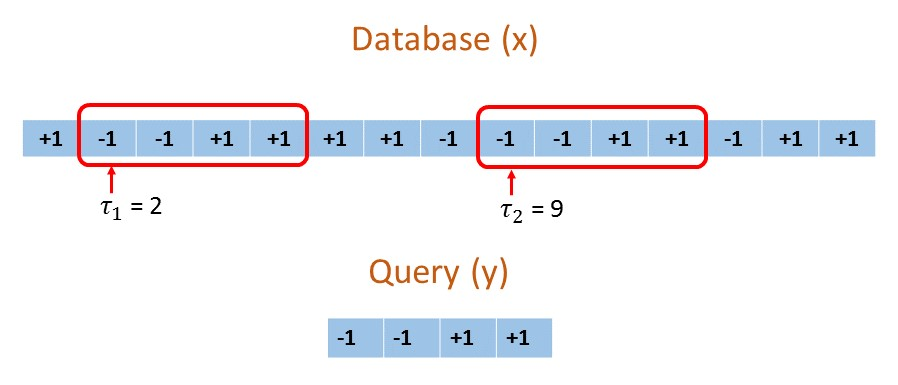
\includegraphics[width=3.4in]{Pattern_matching_ex.jpg}
	\end{figure}
	\vspace{-12pt}
	\begin{block}{}
\begin{itemize}\itemsep3pt
	\item {\color{blue} Database/String}: $\xv = [x[0], x[1], \cdots, x[N]]$ \ (length $N$)
	\item { \color{blue} Query/Substring}: $\yv = [y[0], x[1], \cdots, x[M]]$ \ (length $M = N^\mu$) \vspace{2pt}
	\item Determine all the {\color{blue} $L$ locations} $\underline{\tau} = [\tau_1, \tau_2, \cdots \tau_L]$ with  {\color{blue}high probability}  where\\
	\begin{enumerate}
		\item \normalsize \alert{Exact Matching}:~  $\yv$ appears {\color{blue}exactly} in $\xv$
		\begin{itemize}\normalsize
				\item [-]  $\yv := \xv[\tau:\tau+M-1]$
		\end{itemize}  
		\item \normalsize \alert{Approximate Matching:} ~ $\yv$ is a {\color{blue}noisy substring} of $\xv$
		
		\begin{itemize}\itemsep5pt \normalsize
				\item [-] $\yv := \xv[\tau:\tau+M-1] \odot \bv$ 
				\item [-] $\bv$ is a noise sequence with $d_H(\yv,\xv[\tau:\tau+M-1]) \leq K$   
		\end{itemize}
	\end{enumerate}   
\end{itemize}

	\end{block}
	 \end{frame} 
	 
	 \begin{frame}{Main Result}
	 	
	 \begin{theorem}
	 	Assume that a sketch of $\xv$ of size $O(max(M,N/M)\log N)$ can be precomputed and stored. Then for the {\it exact pattern matching} and {\it approximate pattern matching} (with $K = \eta M,~ 0 \leq \eta \leq 1/6$) problems, with the number of matches $L$ scaling as $O(N^{\lambda})$, our algorithm has
	 	\begin{itemize}
	 		\item a sketching function for $\yv$ that computes {\color{blue} $O(\max(M,\frac{N}{M})\log N)=O(N^{\max(\mu,1-\mu)}\log N)$} \alert{samples}
	 		\item a \alert{computational complexity} of 
	 		\begin{itemize}
	 			% \item  $O(N^{\max(1-\mu,\mu+\lambda)}\log^2 N)$ for $\mu<0.5$
	 			% \item  $O(N^{\max(\mu,1-\mu+\lambda)}\log^2 N)$ for $\mu>0.5$
	 			\item	{\color{blue}$O(\max(N^{1-\mu}\log^2 N, N^{\mu+\lambda}\log N ))$} for {\color{blue}$\mu < 0.5$}
	 			\item	{\color{blue}$O(\max(N^{\mu}\log^2 N, N^{1-\mu +\lambda}\log N ))$} for {\color{blue}$\mu > 0.5$}
	 		\end{itemize}
	 		\item a decoder that recovers all the $L$ matching positions with a {\color{blue}failure probability that approaches zero asymptotically} 
	 	\end{itemize}
	 	
	 	\vspace{10 pt}
	 	{\color{alert}Note:} Particularly when $L=O(1)$ or $L<\frac{N}{M}$ (i.e. $\lambda<1-\mu$) our algorithm has a {\color{blue}sub-linear time} complexity.
	 \end{theorem}	 
\end{frame}	 


\begin{frame} \frametitle{Some Prior Work}
	\vspace{-0.2cm}
	 \begin{block}{\alert{Exact Matching}}
	 	
	 	\begin{itemize}
	 		\item  {\color{blue}\cite{boyer1977fast}}: First occurrence of the match (only $\tau_1$) 
	 		
	 		\begin{itemize}
	 			\item[-] Average complexity - $O(N^{1-\mu} \log N)$ (sublinear)
	 			\item[-] Worst case complexity - $O(N \log N)$  
	 		\end{itemize}
	 	\end{itemize}
	 \end{block}
	\begin{block}{\alert{Approximate Matching}}
		
	 	\begin{itemize}
	 		\item {\color{blue} \cite{chang1994approximate}}: Generalization of \cite{boyer1977fast}
	 		\begin{itemize}
	 			\item[-] Average complexity - $O(NK/M \log N)$ (sub-linear only when $K \ll M$ ) 
	 		\end{itemize}
	 		
	 		\item {\color{blue} \cite{andoni2013shift}}: $O(N/M^{0.359})$ (sub-linear even when $K = O(M)$) 
	 		\begin{itemize}
	 			\item[-] Combinatorial in nature
	 		\end{itemize}
	 	\end{itemize}
	 \end{block}

\begin{block}{\alert{Sparse Fourier Transform Approach}}
	 	\begin{itemize}
	 		\item {\color{blue} \cite{hassanieh2012faster}}: Faster GPS receiver
	 		\begin{itemize}
	 			\item[-] Exploited sparsity in Correlation function $R_{XY}$  
	 		\end{itemize}
	 		
	 		\item {\color{blue} \cite{pawar2014robust}}: Robust Sparse Fourier Transform
	 		\begin{itemize}
	 			\item[-] Sparse Graph code Approach
	 			\item[-] Computational complexity : $O(N \log N)$
	 		\end{itemize}
	 	\end{itemize}	 	
	\end{block}
\end{frame}

\begin{frame}\frametitle{Motivation}
	\vspace{-0.4cm}
			\begin{block}{}
			
				\begin{itemize} 
					\item {\bf Cross-correlation} ($\rv$):
					
					\begin{equation}\label{eqn:Rxy_def} \nonumber
					r[m]=(\xv*\yv)[m] \defeq \sum_{i=0}^{M-1} x[m+i] y[i], ~ ~ \ 0 \leq m \leq N-1  
					\end{equation}
					
					
					\item {\bf Naive implementation}: $O(MN) = O(N^{1+\mu})$ ({\color{blue} super-linear} complexity) 
					
					\item 	{\bf Fourier Transform Approach}: $O(N \log N)$ complexity
					
				\end{itemize}
			\end{block}
			
				\begin{columns}
					\column{0.45\columnwidth}
			\begin{block}{\alert{ \bf Key Observation}}
			\vspace{0.2cm}
				\begin{itemize}
					\item $\rv$ is {\color{blue}Sparse} with some noise.
				\end{itemize}
				  
				 \begin{equation} \label{eqn:RXY_sparse}\nonumber
				 r[m] \ = \left\{
				 \begin{array}{ll}
				 &M,~~  \text{if} \ m \in \mathcal{T} \\
				 & n_m,~~ m \in [N]-\mathcal{T}
				 \end{array} 
				 \right.  
				 \end{equation}
			
			\end{block}
										
					\column[]{0.45\columnwidth}
					\begin{figure}
						\centering
						\scalebox{0.7}{% This file was created by matlab2tikz.
%
%The latest updates can be retrieved from
%  http://www.mathworks.com/matlabcentral/fileexchange/22022-matlab2tikz-matlab2tikz
%where you can also make suggestions and rate matlab2tikz.
%
\definecolor{mycolor1}{rgb}{0.00000,0.44700,0.74100}%
%
\begin{tikzpicture}

\begin{axis}[%
width=4.521in,
height=3.566in,
at={(0.758in,0.481in)},
scale only axis,
xmin=0,
xmax=10000,
xlabel style={font=\color{white!20!black}},
xlabel={Samples},
xtick = {0,2000,4000,6000,8000,10000},
ymin=0,
ymax=100,
ylabel style={font=\color{white!20!black}},
ylabel={Magnitude of Cross-correlation $|R_{XY}|$},
ytick = {0,20,40,60,80,100},
axis background/.style={fill=white}
]
\addplot [color=mycolor1, forget plot, line width=1.5pt]
  table[row sep=crcr]{%
1	0\\
2	0\\
4	2\\
5	0\\
6	0\\
7	1\\
8	0\\
9	4\\
10	0\\
12	0\\
13	1\\
14	0\\
16	0\\
17	1\\
19	1\\
20	0\\
21	1\\
22	0\\
30	0\\
31	1\\
32	1\\
33	2\\
34	0\\
35	0\\
36	1\\
37	0\\
39	0\\
40	1\\
41	0\\
42	0\\
43	1\\
44	1\\
45	0\\
47	0\\
48	1\\
49	0\\
50	0\\
51	2\\
52	0\\
53	0\\
54	1\\
55	0\\
57	0\\
58	2\\
59	0\\
60	0\\
61	1\\
62	0\\
63	0\\
64	1\\
65	0\\
66	1\\
67	0\\
73	0\\
74	1\\
75	0\\
76	1\\
77	0\\
79	0\\
80	1\\
81	0\\
82	0\\
83	2\\
84	0\\
86	2\\
87	1\\
88	1\\
89	2\\
90	0\\
91	0\\
92	1\\
93	0\\
96	0\\
97	2\\
98	0\\
99	0\\
100	2\\
102	0\\
103	3\\
104	0\\
106	0\\
107	1\\
108	0\\
109	0\\
110	2\\
111	0\\
112	1\\
113	1\\
114	0\\
115	1\\
116	0\\
117	0\\
118	2\\
120	0\\
121	2\\
122	0\\
123	2\\
124	0\\
125	1\\
126	0\\
127	0\\
128	1\\
129	1\\
130	0\\
132	0\\
133	1\\
134	0\\
135	0\\
136	1\\
139	1\\
140	0\\
141	0\\
142	1\\
143	1\\
144	2\\
145	1\\
146	1\\
147	0\\
149	0\\
150	2\\
151	0\\
152	0\\
153	1\\
154	0\\
155	0\\
156	1\\
157	0\\
158	1\\
161	1\\
162	0\\
163	0\\
164	1\\
165	0\\
166	4\\
168	0\\
170	0\\
171	2\\
172	0\\
173	1\\
174	0\\
176	0\\
177	2\\
178	0\\
181	0\\
182	1\\
183	0\\
184	0\\
185	2\\
186	0\\
188	2\\
189	0\\
190	1\\
191	0\\
194	0\\
195	1\\
198	1\\
199	0\\
201	0\\
202	1\\
203	0\\
204	1\\
205	0\\
206	2\\
207	0\\
208	1\\
209	0\\
210	1\\
211	0\\
212	2\\
214	0\\
215	1\\
216	0\\
217	2\\
218	2\\
220	0\\
221	1\\
222	0\\
223	1\\
224	0\\
228	0\\
229	1\\
230	0\\
231	1\\
232	0\\
234	0\\
235	1\\
236	1\\
237	0\\
239	0\\
240	1\\
241	0\\
242	1\\
243	0\\
246	0\\
247	2\\
249	0\\
251	0\\
253	2\\
254	1\\
255	1\\
256	0\\
258	0\\
259	1\\
260	0\\
262	0\\
263	1\\
264	0\\
265	1\\
266	0\\
269	0\\
270	1\\
273	1\\
274	2\\
275	0\\
276	1\\
277	0\\
278	0\\
279	1\\
280	0\\
283	0\\
284	2\\
285	2\\
287	0\\
288	2\\
289	0\\
290	1\\
291	0\\
292	0\\
293	1\\
294	0\\
296	0\\
297	1\\
298	0\\
299	1\\
300	0\\
301	0\\
302	2\\
303	0\\
304	0\\
305	1\\
306	0\\
307	0\\
308	2\\
310	0\\
311	1\\
312	0\\
315	0\\
316	1\\
317	1\\
318	0\\
319	0\\
320	1\\
321	1\\
322	0\\
323	2\\
324	0\\
330	0\\
331	1\\
332	1\\
333	0\\
337	0\\
338	2\\
339	0\\
340	1\\
341	0\\
342	0\\
343	2\\
344	0\\
345	2\\
346	0\\
348	0\\
349	1\\
350	0\\
352	0\\
353	1\\
354	0\\
355	1\\
356	0\\
359	0\\
360	1\\
361	0\\
362	0\\
363	1\\
364	0\\
369	0\\
370	1\\
371	0\\
372	1\\
373	1\\
374	0\\
375	2\\
376	0\\
377	1\\
378	0\\
379	2\\
380	0\\
381	1\\
382	0\\
383	0\\
384	1\\
385	0\\
386	1\\
387	0\\
388	1\\
389	0\\
390	0\\
392	2\\
393	0\\
395	0\\
396	1\\
397	0\\
398	1\\
399	0\\
400	1\\
401	0\\
403	0\\
404	1\\
406	1\\
407	0\\
409	0\\
410	2\\
411	0\\
412	0\\
413	2\\
414	0\\
415	2\\
416	0\\
423	0\\
424	2\\
425	0\\
426	0\\
427	2\\
428	0\\
429	2\\
430	0\\
431	0\\
432	1\\
433	0\\
437	0\\
438	1\\
439	1\\
440	2\\
441	1\\
442	2\\
443	0\\
446	0\\
447	1\\
448	1\\
449	0\\
451	0\\
452	2\\
453	1\\
454	1\\
455	0\\
456	1\\
457	1\\
458	0\\
459	0\\
460	1\\
461	0\\
462	0\\
463	2\\
464	0\\
467	0\\
468	1\\
470	1\\
471	0\\
472	1\\
473	1\\
474	3\\
475	0\\
476	1\\
478	1\\
479	2\\
480	0\\
481	1\\
482	1\\
483	0\\
488	0\\
489	1\\
490	1\\
491	0\\
492	1\\
493	0\\
494	1\\
495	0\\
498	0\\
499	3\\
500	1\\
501	0\\
506	0\\
507	2\\
508	0\\
509	2\\
510	2\\
511	0\\
513	2\\
514	0\\
515	2\\
517	0\\
518	2\\
519	0\\
523	0\\
524	1\\
525	0\\
526	1\\
528	1\\
529	0\\
530	0\\
531	2\\
532	0\\
537	0\\
538	1\\
539	0\\
541	0\\
542	1\\
543	1\\
544	2\\
546	0\\
547	1\\
548	0\\
553	0\\
554	1\\
555	0\\
556	0\\
557	2\\
558	0\\
560	2\\
561	1\\
562	1\\
563	0\\
564	0\\
565	1\\
566	1\\
567	0\\
568	1\\
569	1\\
570	0\\
571	0\\
572	1\\
574	1\\
575	0\\
578	0\\
579	1\\
580	0\\
581	0\\
582	2\\
583	2\\
585	0\\
587	0\\
588	1\\
589	0\\
591	0\\
592	1\\
593	0\\
594	0\\
595	1\\
598	1\\
599	0\\
601	0\\
602	1\\
603	1\\
604	0\\
605	1\\
607	1\\
608	0\\
609	0\\
610	1\\
611	0\\
612	1\\
614	1\\
615	0\\
616	1\\
617	0\\
618	1\\
619	0\\
620	2\\
621	0\\
622	1\\
623	0\\
624	3\\
625	0\\
626	1\\
627	1\\
628	0\\
629	0\\
630	1\\
631	0\\
632	1\\
633	1\\
634	0\\
637	0\\
638	1\\
639	0\\
640	1\\
641	0\\
642	2\\
643	0\\
644	0\\
645	2\\
646	0\\
649	0\\
651	2\\
652	0\\
654	0\\
655	2\\
657	0\\
658	0\\
659	1\\
660	0\\
661	0\\
662	1\\
663	3\\
664	0\\
665	0\\
666	1\\
667	0\\
668	1\\
673	1\\
674	0\\
675	0\\
676	2\\
677	0\\
678	0\\
679	1\\
680	0\\
681	3\\
682	0\\
685	0\\
686	2\\
687	0\\
688	1\\
689	0\\
690	3\\
691	1\\
692	0\\
693	1\\
695	1\\
696	0\\
697	0\\
698	1\\
699	1\\
700	3\\
701	0\\
702	1\\
703	0\\
707	0\\
708	1\\
709	1\\
710	2\\
711	0\\
714	0\\
715	1\\
716	0\\
717	0\\
718	1\\
719	0\\
720	1\\
721	1\\
722	3\\
723	0\\
725	0\\
726	2\\
727	0\\
729	0\\
730	3\\
731	0\\
732	0\\
733	1\\
734	0\\
736	0\\
737	1\\
738	1\\
739	2\\
741	0\\
743	0\\
744	2\\
745	0\\
746	0\\
747	1\\
748	0\\
752	0\\
753	2\\
755	0\\
757	0\\
758	1\\
762	1\\
763	0\\
764	1\\
765	0\\
768	0\\
770	2\\
771	0\\
778	0\\
779	1\\
780	0\\
783	0\\
784	3\\
785	1\\
786	0\\
791	0\\
792	4\\
793	1\\
794	0\\
796	0\\
797	2\\
798	0\\
801	0\\
802	1\\
803	0\\
808	0\\
809	1\\
810	1\\
811	0\\
812	0\\
814	2\\
815	0\\
816	1\\
817	1\\
818	0\\
819	0\\
820	2\\
821	0\\
822	0\\
823	1\\
824	0\\
825	0\\
826	1\\
827	0\\
828	2\\
829	0\\
830	1\\
831	1\\
832	0\\
833	0\\
834	1\\
835	0\\
836	0\\
837	1\\
838	0\\
839	2\\
841	0\\
842	0\\
843	1\\
844	0\\
845	1\\
846	0\\
848	0\\
849	1\\
850	0\\
851	1\\
852	1\\
853	0\\
854	1\\
855	0\\
856	0\\
857	1\\
858	1\\
859	2\\
860	0\\
861	1\\
862	0\\
868	0\\
869	1\\
870	0\\
871	0\\
872	2\\
873	1\\
876	1\\
877	0\\
878	1\\
879	1\\
880	0\\
883	0\\
884	1\\
885	0\\
886	2\\
888	0\\
892	0\\
893	2\\
894	0\\
895	3\\
896	2\\
897	2\\
898	0\\
899	0\\
900	1\\
901	1\\
902	0\\
909	0\\
910	93\\
911	0\\
912	0\\
913	1\\
914	0\\
920	0\\
921	1\\
922	0\\
923	0\\
924	3\\
925	1\\
926	2\\
928	2\\
929	0\\
932	0\\
933	2\\
934	0\\
941	0\\
942	1\\
943	1\\
944	0\\
945	2\\
946	2\\
947	0\\
951	0\\
952	1\\
953	0\\
957	0\\
958	1\\
959	0\\
960	2\\
961	0\\
963	2\\
964	0\\
965	1\\
966	1\\
967	0\\
970	0\\
971	1\\
972	0\\
976	0\\
977	2\\
978	0\\
979	0\\
980	1\\
981	1\\
982	0\\
983	1\\
984	1\\
985	0\\
989	0\\
990	1\\
991	1\\
992	0\\
993	1\\
994	1\\
995	2\\
996	0\\
999	0\\
1000	3\\
1001	0\\
1004	0\\
1005	1\\
1006	0\\
1007	0\\
1008	1\\
1009	0\\
1010	1\\
1011	0\\
1012	1\\
1013	0\\
1014	1\\
1015	1\\
1016	0\\
1017	2\\
1018	0\\
1019	1\\
1020	0\\
1022	0\\
1023	1\\
1024	0\\
1025	0\\
1027	2\\
1029	0\\
1030	0\\
1031	1\\
1032	0\\
1033	1\\
1034	0\\
1035	0\\
1036	1\\
1037	0\\
1040	0\\
1041	1\\
1042	0\\
1044	2\\
1045	0\\
1046	0\\
1047	1\\
1048	1\\
1049	0\\
1050	1\\
1051	0\\
1052	1\\
1053	0\\
1054	1\\
1055	1\\
1056	0\\
1057	0\\
1058	1\\
1059	0\\
1063	0\\
1064	2\\
1065	0\\
1066	0\\
1067	2\\
1068	0\\
1071	0\\
1072	1\\
1073	1\\
1074	2\\
1075	0\\
1076	1\\
1077	0\\
1078	1\\
1079	0\\
1080	0\\
1082	2\\
1083	0\\
1084	2\\
1085	0\\
1092	0\\
1093	1\\
1094	0\\
1096	0\\
1097	2\\
1098	0\\
1099	0\\
1100	1\\
1101	0\\
1102	6\\
1103	1\\
1104	0\\
1105	1\\
1106	0\\
1107	0\\
1108	1\\
1109	0\\
1111	0\\
1112	1\\
1113	0\\
1115	0\\
1117	2\\
1118	0\\
1119	1\\
1120	0\\
1124	0\\
1125	1\\
1126	0\\
1130	0\\
1131	2\\
1132	0\\
1134	2\\
1136	0\\
1137	2\\
1139	0\\
1143	0\\
1144	1\\
1145	0\\
1151	0\\
1152	1\\
1153	1\\
1154	0\\
1156	0\\
1157	1\\
1158	0\\
1159	2\\
1160	0\\
1164	0\\
1165	2\\
1166	1\\
1167	1\\
1168	0\\
1169	1\\
1170	0\\
1174	0\\
1175	1\\
1176	0\\
1183	0\\
1184	1\\
1185	0\\
1186	2\\
1187	2\\
1188	0\\
1192	0\\
1193	1\\
1194	0\\
1196	0\\
1197	1\\
1198	0\\
1199	0\\
1200	2\\
1201	0\\
1202	1\\
1203	0\\
1206	0\\
1207	1\\
1208	0\\
1209	1\\
1212	1\\
1213	0\\
1214	1\\
1215	0\\
1216	1\\
1217	1\\
1218	0\\
1219	1\\
1220	0\\
1223	0\\
1224	1\\
1226	1\\
1227	0\\
1228	1\\
1229	0\\
1231	0\\
1232	1\\
1233	0\\
1237	0\\
1238	1\\
1239	0\\
1240	2\\
1241	0\\
1245	0\\
1246	1\\
1247	0\\
1248	0\\
1249	2\\
1250	0\\
1251	1\\
1252	0\\
1253	0\\
1254	1\\
1255	0\\
1257	0\\
1258	1\\
1259	0\\
1260	2\\
1261	1\\
1262	1\\
1263	0\\
1264	0\\
1265	2\\
1266	0\\
1267	0\\
1268	1\\
1269	0\\
1270	0\\
1271	2\\
1273	0\\
1274	3\\
1275	0\\
1276	0\\
1277	2\\
1278	0\\
1279	0\\
1280	2\\
1281	0\\
1282	2\\
1284	0\\
1285	0\\
1286	1\\
1287	0\\
1288	1\\
1289	0\\
1292	0\\
1293	1\\
1294	0\\
1297	0\\
1298	1\\
1299	0\\
1303	0\\
1304	1\\
1305	0\\
1306	1\\
1307	3\\
1308	1\\
1309	0\\
1317	0\\
1318	1\\
1319	1\\
1320	0\\
1321	0\\
1322	1\\
1323	0\\
1324	1\\
1325	0\\
1329	0\\
1330	1\\
1331	0\\
1332	1\\
1333	0\\
1334	1\\
1335	0\\
1338	0\\
1339	1\\
1341	1\\
1342	2\\
1343	0\\
1347	0\\
1348	1\\
1349	0\\
1350	0\\
1351	1\\
1352	3\\
1353	1\\
1354	1\\
1355	0\\
1356	0\\
1358	2\\
1359	0\\
1360	1\\
1361	0\\
1362	1\\
1363	0\\
1364	0\\
1365	1\\
1366	0\\
1370	0\\
1371	1\\
1372	1\\
1373	0\\
1374	0\\
1375	1\\
1376	0\\
1379	0\\
1380	1\\
1381	0\\
1382	1\\
1383	0\\
1384	0\\
1385	1\\
1386	0\\
1387	0\\
1389	2\\
1391	0\\
1392	1\\
1393	0\\
1396	0\\
1397	1\\
1398	0\\
1399	2\\
1400	0\\
1405	0\\
1406	2\\
1407	0\\
1413	0\\
1414	1\\
1415	1\\
1416	0\\
1422	0\\
1423	1\\
1424	0\\
1428	0\\
1429	1\\
1430	0\\
1431	0\\
1432	1\\
1433	1\\
1434	0\\
1436	0\\
1437	1\\
1438	0\\
1444	0\\
1445	1\\
1446	0\\
1447	2\\
1448	0\\
1450	0\\
1452	2\\
1453	0\\
1456	0\\
1458	2\\
1459	0\\
1460	1\\
1461	0\\
1463	0\\
1464	1\\
1465	0\\
1466	1\\
1468	1\\
1469	0\\
1470	1\\
1471	0\\
1476	0\\
1477	2\\
1478	0\\
1479	1\\
1480	0\\
1481	1\\
1482	1\\
1483	0\\
1484	0\\
1485	3\\
1486	1\\
1487	0\\
1491	0\\
1493	2\\
1494	2\\
1495	1\\
1496	1\\
1497	0\\
1498	1\\
1499	0\\
1500	0\\
1501	1\\
1502	0\\
1507	0\\
1508	1\\
1509	1\\
1510	0\\
1511	0\\
1512	1\\
1513	0\\
1514	1\\
1515	3\\
1516	1\\
1517	1\\
1518	0\\
1521	0\\
1522	2\\
1523	0\\
1525	0\\
1526	2\\
1527	0\\
1528	0\\
1529	1\\
1532	1\\
1533	0\\
1535	0\\
1536	2\\
1538	0\\
1539	0\\
1540	1\\
1541	1\\
1542	0\\
1543	0\\
1544	1\\
1546	1\\
1547	0\\
1548	1\\
1549	1\\
1550	0\\
1551	1\\
1552	3\\
1553	0\\
1554	2\\
1555	0\\
1560	0\\
1561	3\\
1562	0\\
1564	2\\
1566	0\\
1567	1\\
1570	1\\
1571	0\\
1573	0\\
1575	2\\
1576	0\\
1577	0\\
1578	3\\
1579	0\\
1580	1\\
1581	0\\
1582	1\\
1583	0\\
1584	3\\
1585	0\\
1588	0\\
1589	1\\
1590	1\\
1591	0\\
1592	1\\
1593	0\\
1596	0\\
1597	1\\
1598	0\\
1599	1\\
1600	0\\
1601	2\\
1602	0\\
1603	1\\
1604	0\\
1605	0\\
1606	1\\
1607	1\\
1608	0\\
1609	0\\
1610	1\\
1611	0\\
1614	0\\
1615	1\\
1616	0\\
1619	0\\
1620	1\\
1621	0\\
1633	0\\
1634	1\\
1635	0\\
1639	0\\
1640	1\\
1641	0\\
1642	0\\
1643	1\\
1644	0\\
1645	0\\
1646	1\\
1647	1\\
1648	0\\
1652	0\\
1653	1\\
1654	0\\
1657	0\\
1658	1\\
1659	0\\
1660	1\\
1661	0\\
1662	0\\
1663	1\\
1665	1\\
1666	0\\
1669	0\\
1670	1\\
1671	0\\
1673	0\\
1674	1\\
1675	0\\
1676	1\\
1677	0\\
1678	1\\
1679	1\\
1680	0\\
1681	1\\
1682	0\\
1689	0\\
1690	1\\
1691	4\\
1692	0\\
1695	0\\
1696	1\\
1697	1\\
1698	0\\
1700	0\\
1701	1\\
1702	0\\
1707	0\\
1708	1\\
1709	0\\
1716	0\\
1717	2\\
1718	1\\
1719	1\\
1720	0\\
1721	1\\
1722	0\\
1727	0\\
1728	1\\
1729	1\\
1730	0\\
1734	0\\
1735	1\\
1736	0\\
1739	0\\
1740	1\\
1741	0\\
1742	3\\
1743	0\\
1752	0\\
1753	1\\
1754	0\\
1755	0\\
1756	1\\
1757	0\\
1758	0\\
1759	1\\
1760	0\\
1761	0\\
1762	1\\
1763	0\\
1764	1\\
1765	1\\
1766	0\\
1767	1\\
1768	0\\
1769	0\\
1770	1\\
1771	0\\
1773	0\\
1774	1\\
1775	0\\
1777	0\\
1778	1\\
1779	1\\
1780	0\\
1781	2\\
1782	0\\
1790	0\\
1791	1\\
1792	0\\
1793	0\\
1794	1\\
1795	0\\
1799	0\\
1800	2\\
1801	0\\
1802	1\\
1803	0\\
1805	0\\
1806	1\\
1807	0\\
1808	1\\
1809	3\\
1810	0\\
1811	1\\
1812	0\\
1813	2\\
1814	0\\
1817	0\\
1818	1\\
1819	1\\
1820	0\\
1821	1\\
1822	0\\
1825	0\\
1826	1\\
1827	0\\
1828	1\\
1829	0\\
1831	0\\
1832	1\\
1833	0\\
1834	0\\
1835	1\\
1836	0\\
1841	0\\
1842	1\\
1843	0\\
1845	0\\
1846	1\\
1848	1\\
1849	0\\
1850	2\\
1851	0\\
1852	1\\
1853	0\\
1859	0\\
1860	1\\
1861	0\\
1862	0\\
1863	1\\
1864	0\\
1865	1\\
1866	0\\
1869	0\\
1870	1\\
1871	0\\
1877	0\\
1878	1\\
1880	1\\
1881	0\\
1882	1\\
1883	0\\
1886	0\\
1887	1\\
1888	0\\
1889	1\\
1890	0\\
1891	0\\
1892	1\\
1893	1\\
1894	0\\
1895	1\\
1896	0\\
1897	2\\
1898	0\\
1899	1\\
1900	0\\
1903	0\\
1904	1\\
1905	0\\
1910	0\\
1912	2\\
1913	0\\
1914	1\\
1915	0\\
1917	0\\
1918	1\\
1919	0\\
1920	2\\
1921	0\\
1922	0\\
1923	1\\
1924	0\\
1925	1\\
1926	0\\
1927	4\\
1928	1\\
1929	0\\
1930	0\\
1931	1\\
1932	0\\
1933	0\\
1934	2\\
1935	0\\
1936	1\\
1937	0\\
1938	0\\
1939	1\\
1940	0\\
1943	0\\
1944	2\\
1945	0\\
1948	0\\
1949	1\\
1950	1\\
1951	0\\
1953	2\\
1955	0\\
1956	1\\
1957	0\\
1959	0\\
1960	1\\
1961	0\\
1962	1\\
1963	0\\
1968	0\\
1969	3\\
1970	0\\
1971	1\\
1972	0\\
1973	1\\
1974	0\\
1975	1\\
1976	1\\
1977	4\\
1978	0\\
1981	0\\
1982	1\\
1983	0\\
1986	0\\
1988	2\\
1989	0\\
1990	1\\
1991	0\\
1992	0\\
1993	2\\
1994	0\\
1997	0\\
1998	1\\
1999	0\\
2003	0\\
2004	2\\
2005	1\\
2006	1\\
2007	0\\
2009	0\\
2010	1\\
2011	0\\
2012	2\\
2013	0\\
2016	0\\
2017	1\\
2018	0\\
2024	0\\
2025	1\\
2026	0\\
2027	0\\
2028	1\\
2029	0\\
2030	2\\
2031	0\\
2032	1\\
2033	0\\
2034	2\\
2035	0\\
2036	1\\
2037	1\\
2038	0\\
2041	0\\
2042	1\\
2043	0\\
2046	0\\
2047	3\\
2048	0\\
2057	0\\
2058	1\\
2059	0\\
2060	1\\
2061	1\\
2062	0\\
2068	0\\
2069	1\\
2070	0\\
2071	1\\
2072	0\\
2076	0\\
2077	3\\
2079	3\\
2080	1\\
2081	0\\
2082	0\\
2083	1\\
2084	0\\
2087	0\\
2088	1\\
2089	0\\
2090	0\\
2091	1\\
2092	1\\
2093	0\\
2095	0\\
2096	1\\
2097	1\\
2098	0\\
2107	0\\
2108	1\\
2109	0\\
2110	0\\
2111	1\\
2112	0\\
2113	0\\
2114	1\\
2115	0\\
2124	0\\
2125	1\\
2126	0\\
2127	1\\
2128	0\\
2129	1\\
2131	1\\
2133	3\\
2134	0\\
2135	0\\
2136	1\\
2137	0\\
2139	0\\
2140	1\\
2141	1\\
2142	0\\
2146	0\\
2147	1\\
2148	0\\
2149	0\\
2150	1\\
2151	0\\
2152	1\\
2153	0\\
2154	0\\
2155	1\\
2156	0\\
2160	0\\
2161	1\\
2162	0\\
2163	0\\
2164	1\\
2165	0\\
2166	1\\
2167	0\\
2168	0\\
2169	1\\
2170	0\\
2171	0\\
2172	1\\
2173	0\\
2178	0\\
2179	2\\
2180	0\\
2181	0\\
2182	1\\
2183	0\\
2191	0\\
2192	1\\
2193	0\\
2197	0\\
2198	1\\
2199	0\\
2207	0\\
2208	2\\
2209	0\\
2212	0\\
2213	1\\
2214	0\\
2219	0\\
2220	1\\
2221	0\\
2223	0\\
2224	1\\
2225	1\\
2226	0\\
2227	0\\
2228	2\\
2229	0\\
2230	1\\
2231	0\\
2237	0\\
2238	3\\
2239	0\\
2240	1\\
2241	0\\
2242	0\\
2243	1\\
2244	0\\
2245	2\\
2246	0\\
2247	1\\
2248	0\\
2249	0\\
2250	1\\
2252	1\\
2253	0\\
2255	0\\
2256	1\\
2257	1\\
2258	0\\
2259	1\\
2260	0\\
2262	0\\
2263	2\\
2264	0\\
2266	0\\
2267	1\\
2268	0\\
2270	0\\
2271	2\\
2272	1\\
2273	1\\
2274	0\\
2276	0\\
2277	1\\
2278	0\\
2280	0\\
2281	1\\
2282	0\\
2283	0\\
2284	1\\
2285	0\\
2286	1\\
2287	0\\
2289	0\\
2290	1\\
2291	1\\
2292	0\\
2293	0\\
2295	2\\
2296	0\\
2298	0\\
2299	1\\
2300	0\\
2303	0\\
2304	1\\
2306	1\\
2307	0\\
2308	2\\
2309	0\\
2310	1\\
2311	0\\
2312	0\\
2313	1\\
2314	0\\
2316	0\\
2317	1\\
2318	0\\
2319	1\\
2320	0\\
2321	1\\
2322	0\\
2325	0\\
2326	3\\
2327	1\\
2328	0\\
2329	0\\
2330	2\\
2331	0\\
2333	0\\
2334	3\\
2335	0\\
2337	0\\
2338	1\\
2339	0\\
2340	1\\
2341	1\\
2342	0\\
2343	1\\
2344	0\\
2345	1\\
2346	0\\
2347	1\\
2348	1\\
2349	0\\
2352	0\\
2353	1\\
2354	0\\
2356	0\\
2357	1\\
2358	0\\
2360	0\\
2361	3\\
2362	1\\
2363	0\\
2366	0\\
2367	1\\
2368	0\\
2369	2\\
2370	2\\
2371	0\\
2372	0\\
2373	1\\
2374	0\\
2375	1\\
2376	0\\
2377	0\\
2378	3\\
2379	0\\
2380	1\\
2381	0\\
2382	1\\
2383	0\\
2384	0\\
2385	1\\
2386	0\\
2389	0\\
2390	1\\
2391	1\\
2392	0\\
2396	0\\
2397	1\\
2399	1\\
2400	0\\
2404	0\\
2405	1\\
2406	0\\
2407	0\\
2408	2\\
2409	1\\
2411	1\\
2412	0\\
2413	1\\
2414	0\\
2415	0\\
2416	1\\
2417	0\\
2419	0\\
2421	2\\
2422	0\\
2436	0\\
2437	1\\
2438	0\\
2445	0\\
2446	1\\
2447	0\\
2451	0\\
2452	1\\
2453	0\\
2459	0\\
2461	2\\
2462	0\\
2467	0\\
2468	1\\
2469	0\\
2472	0\\
2473	2\\
2474	0\\
2475	0\\
2476	1\\
2477	0\\
2478	0\\
2479	1\\
2480	0\\
2481	2\\
2482	0\\
2483	1\\
2484	0\\
2485	0\\
2486	4\\
2487	0\\
2492	0\\
2493	1\\
2494	0\\
2495	0\\
2496	1\\
2499	1\\
2500	3\\
2501	0\\
2503	0\\
2504	2\\
2505	0\\
2507	0\\
2508	2\\
2510	0\\
2511	1\\
2512	0\\
2516	0\\
2517	1\\
2518	1\\
2519	3\\
2520	4\\
2521	0\\
2522	2\\
2523	3\\
2524	0\\
2526	0\\
2527	1\\
2528	0\\
2529	1\\
2530	0\\
2531	2\\
2532	0\\
2535	0\\
2536	1\\
2537	0\\
2538	1\\
2539	0\\
2540	0\\
2541	1\\
2542	0\\
2543	0\\
2544	4\\
2545	0\\
2549	0\\
2550	1\\
2551	0\\
2552	0\\
2553	1\\
2554	0\\
2558	0\\
2559	1\\
2560	0\\
2562	0\\
2563	2\\
2564	0\\
2565	0\\
2566	1\\
2567	1\\
2568	0\\
2569	1\\
2570	1\\
2571	0\\
2572	0\\
2573	1\\
2574	1\\
2575	0\\
2576	1\\
2577	0\\
2579	2\\
2580	2\\
2581	0\\
2582	1\\
2583	0\\
2584	2\\
2586	0\\
2587	1\\
2588	0\\
2590	0\\
2591	1\\
2592	0\\
2593	1\\
2594	0\\
2595	0\\
2596	1\\
2597	0\\
2599	2\\
2600	0\\
2601	0\\
2602	1\\
2603	1\\
2604	0\\
2605	0\\
2606	1\\
2607	0\\
2610	0\\
2612	2\\
2614	0\\
2615	1\\
2616	1\\
2617	0\\
2619	0\\
2620	1\\
2622	1\\
2623	0\\
2625	0\\
2626	2\\
2627	0\\
2628	1\\
2629	1\\
2630	0\\
2631	0\\
2632	2\\
2634	0\\
2635	0\\
2636	2\\
2637	0\\
2638	1\\
2639	0\\
2642	0\\
2643	1\\
2644	1\\
2645	0\\
2646	1\\
2647	0\\
2648	0\\
2650	2\\
2651	0\\
2652	0\\
2653	1\\
2654	0\\
2656	0\\
2657	1\\
2658	1\\
2659	0\\
2662	0\\
2663	2\\
2664	1\\
2668	1\\
2669	0\\
2670	1\\
2671	0\\
2674	0\\
2675	2\\
2676	0\\
2677	2\\
2678	0\\
2679	1\\
2680	1\\
2681	0\\
2691	0\\
2693	2\\
2694	0\\
2695	0\\
2696	1\\
2697	1\\
2698	0\\
2699	2\\
2700	0\\
2701	1\\
2702	0\\
2703	1\\
2704	0\\
2705	0\\
2706	1\\
2707	1\\
2708	0\\
2709	0\\
2710	3\\
2711	0\\
2712	1\\
2713	0\\
2715	0\\
2716	1\\
2717	3\\
2718	0\\
2719	0\\
2720	2\\
2721	0\\
2722	2\\
2723	0\\
2724	0\\
2725	1\\
2726	0\\
2727	2\\
2729	0\\
2730	1\\
2731	3\\
2732	2\\
2733	0\\
2735	0\\
2736	1\\
2737	1\\
2738	0\\
2739	0\\
2740	2\\
2741	0\\
2742	0\\
2743	1\\
2744	0\\
2747	0\\
2748	1\\
2749	4\\
2750	0\\
2753	0\\
2754	1\\
2755	1\\
2756	2\\
2757	0\\
2758	2\\
2759	0\\
2760	3\\
2761	0\\
2764	0\\
2766	2\\
2767	0\\
2768	2\\
2769	0\\
2770	1\\
2771	0\\
2772	1\\
2773	0\\
2775	0\\
2776	2\\
2777	1\\
2778	1\\
2779	0\\
2780	2\\
2782	0\\
2783	1\\
2784	0\\
2785	1\\
2786	0\\
2788	0\\
2789	1\\
2790	0\\
2792	0\\
2793	1\\
2794	0\\
2795	1\\
2796	0\\
2798	0\\
2799	1\\
2800	0\\
2801	1\\
2802	0\\
2803	1\\
2804	0\\
2805	0\\
2807	2\\
2808	0\\
2809	1\\
2810	0\\
2811	1\\
2812	1\\
2813	0\\
2814	0\\
2815	1\\
2816	1\\
2817	0\\
2818	0\\
2819	1\\
2820	0\\
2821	1\\
2822	0\\
2823	0\\
2824	2\\
2825	3\\
2826	0\\
2827	1\\
2828	0\\
2829	1\\
2830	0\\
2831	2\\
2832	0\\
2833	1\\
2834	0\\
2835	2\\
2836	0\\
2837	1\\
2838	0\\
2841	0\\
2842	1\\
2843	1\\
2844	0\\
2845	1\\
2846	0\\
2847	1\\
2848	0\\
2849	2\\
2850	0\\
2851	0\\
2852	2\\
2854	0\\
2855	1\\
2856	1\\
2857	0\\
2859	0\\
2860	3\\
2861	0\\
2868	0\\
2869	1\\
2870	1\\
2871	0\\
2873	0\\
2874	3\\
2875	1\\
2876	2\\
2877	2\\
2878	0\\
2879	0\\
2881	2\\
2882	0\\
2883	0\\
2884	1\\
2885	0\\
2886	0\\
2888	2\\
2889	1\\
2890	1\\
2891	0\\
2892	1\\
2893	0\\
2895	0\\
2896	1\\
2897	0\\
2898	1\\
2899	0\\
2900	2\\
2901	0\\
2902	1\\
2903	0\\
2904	0\\
2905	2\\
2906	0\\
2907	0\\
2908	3\\
2909	0\\
2911	0\\
2912	2\\
2913	0\\
2914	0\\
2915	1\\
2916	1\\
2917	0\\
2919	0\\
2921	2\\
2923	0\\
2928	0\\
2929	4\\
2930	0\\
2931	0\\
2932	1\\
2933	1\\
2934	0\\
2935	1\\
2936	0\\
2937	0\\
2938	2\\
2939	1\\
2940	1\\
2941	0\\
2942	0\\
2944	2\\
2945	0\\
2951	0\\
2952	2\\
2953	0\\
2956	0\\
2958	2\\
2959	1\\
2960	1\\
2961	0\\
2962	1\\
2963	1\\
2964	0\\
2965	0\\
2966	1\\
2967	1\\
2968	0\\
2970	0\\
2971	1\\
2972	0\\
2974	0\\
2975	2\\
2977	0\\
2978	1\\
2979	0\\
2983	0\\
2984	1\\
2985	0\\
2986	1\\
2987	1\\
2988	0\\
2989	2\\
2990	0\\
2991	0\\
2992	1\\
2993	0\\
2994	0\\
2995	5\\
2996	0\\
3002	0\\
3003	1\\
3004	1\\
3005	0\\
3006	0\\
3007	3\\
3008	1\\
3009	0\\
3010	1\\
3011	1\\
3012	0\\
3022	0\\
3024	2\\
3025	0\\
3026	3\\
3028	1\\
3029	1\\
3030	0\\
3032	0\\
3033	1\\
3034	0\\
3037	0\\
3038	1\\
3039	0\\
3040	0\\
3041	1\\
3042	0\\
3044	0\\
3045	1\\
3046	0\\
3047	0\\
3048	1\\
3049	0\\
3050	1\\
3051	0\\
3055	0\\
3056	1\\
3057	1\\
3058	0\\
3059	2\\
3060	0\\
3061	0\\
3062	2\\
3063	0\\
3064	2\\
3065	0\\
3066	3\\
3067	1\\
3068	1\\
3069	0\\
3070	1\\
3071	0\\
3074	0\\
3075	1\\
3076	0\\
3077	1\\
3078	0\\
3079	1\\
3080	1\\
3081	0\\
3083	0\\
3084	1\\
3085	0\\
3086	0\\
3087	2\\
3088	0\\
3089	1\\
3091	1\\
3092	0\\
3093	1\\
3094	0\\
3097	0\\
3098	1\\
3099	0\\
3101	2\\
3103	0\\
3104	2\\
3106	0\\
3108	2\\
3109	0\\
3110	1\\
3111	1\\
3112	2\\
3113	0\\
3118	0\\
3119	2\\
3120	0\\
3121	1\\
3122	0\\
3123	0\\
3124	1\\
3125	0\\
3126	0\\
3127	2\\
3128	1\\
3129	2\\
3131	0\\
3132	0\\
3133	3\\
3134	0\\
3135	1\\
3136	0\\
3137	0\\
3138	1\\
3139	0\\
3140	1\\
3144	1\\
3145	0\\
3146	0\\
3147	3\\
3148	0\\
3149	0\\
3150	3\\
3151	0\\
3152	0\\
3153	1\\
3154	0\\
3158	0\\
3159	1\\
3160	3\\
3161	0\\
3164	0\\
3165	2\\
3166	0\\
3173	0\\
3174	1\\
3175	0\\
3177	0\\
3178	1\\
3179	0\\
3182	0\\
3183	1\\
3184	0\\
3191	0\\
3192	1\\
3193	0\\
3196	0\\
3197	1\\
3198	1\\
3199	0\\
3200	2\\
3201	0\\
3202	0\\
3203	1\\
3204	0\\
3212	0\\
3213	1\\
3214	1\\
3215	0\\
3216	1\\
3217	3\\
3218	0\\
3222	0\\
3223	1\\
3224	1\\
3225	0\\
3227	2\\
3228	2\\
3229	0\\
3230	1\\
3231	1\\
3232	0\\
3233	0\\
3234	1\\
3235	0\\
3241	0\\
3242	1\\
3243	0\\
3244	3\\
3245	1\\
3246	1\\
3247	0\\
3251	0\\
3252	1\\
3253	0\\
3254	1\\
3255	0\\
3256	1\\
3257	0\\
3258	1\\
3259	1\\
3260	0\\
3261	0\\
3262	1\\
3263	0\\
3264	2\\
3265	0\\
3266	1\\
3267	0\\
3271	0\\
3272	1\\
3273	1\\
3274	0\\
3275	2\\
3276	2\\
3277	0\\
3278	1\\
3279	1\\
3280	3\\
3281	1\\
3283	1\\
3284	0\\
3286	0\\
3287	1\\
3288	1\\
3289	0\\
3293	0\\
3294	2\\
3295	0\\
3296	0\\
3297	3\\
3298	0\\
3300	0\\
3301	1\\
3302	0\\
3304	0\\
3305	1\\
3306	0\\
3308	0\\
3309	1\\
3310	0\\
3311	1\\
3312	0\\
3313	1\\
3314	1\\
3315	0\\
3316	1\\
3317	1\\
3318	0\\
3322	0\\
3323	1\\
3324	0\\
3325	0\\
3326	3\\
3329	0\\
3330	0\\
3331	2\\
3332	0\\
3333	1\\
3334	0\\
3335	1\\
3336	1\\
3337	2\\
3338	0\\
3339	2\\
3341	0\\
3342	1\\
3343	0\\
3344	2\\
3345	0\\
3348	0\\
3349	2\\
3350	0\\
3357	0\\
3358	1\\
3359	0\\
3361	0\\
3362	1\\
3363	1\\
3364	0\\
3365	0\\
3366	1\\
3367	0\\
3368	1\\
3369	0\\
3370	0\\
3371	1\\
3372	0\\
3380	0\\
3381	1\\
3382	0\\
3387	0\\
3388	1\\
3389	0\\
3390	1\\
3391	0\\
3400	0\\
3401	1\\
3402	1\\
3403	0\\
3404	0\\
3405	1\\
3406	0\\
3407	1\\
3408	0\\
3415	0\\
3416	2\\
3417	0\\
3418	1\\
3419	0\\
3420	0\\
3421	1\\
3422	0\\
3423	0\\
3425	2\\
3426	0\\
3427	2\\
3428	0\\
3429	0\\
3430	2\\
3432	0\\
3435	0\\
3436	2\\
3438	0\\
3439	1\\
3440	0\\
3441	1\\
3442	1\\
3443	0\\
3444	1\\
3446	1\\
3447	0\\
3448	2\\
3449	0\\
3454	0\\
3455	2\\
3456	0\\
3457	1\\
3458	1\\
3459	2\\
3460	0\\
3461	1\\
3462	0\\
3465	0\\
3466	1\\
3467	0\\
3468	0\\
3469	1\\
3470	0\\
3471	0\\
3472	1\\
3473	0\\
3474	1\\
3475	0\\
3476	1\\
3477	1\\
3478	0\\
3479	1\\
3480	0\\
3482	0\\
3483	1\\
3485	1\\
3486	0\\
3487	0\\
3488	1\\
3489	1\\
3490	0\\
3492	0\\
3493	2\\
3494	0\\
3495	0\\
3496	1\\
3497	1\\
3498	0\\
3500	2\\
3501	0\\
3502	1\\
3503	0\\
3504	0\\
3505	1\\
3507	1\\
3508	0\\
3509	1\\
3510	0\\
3512	2\\
3513	0\\
3514	1\\
3515	1\\
3516	0\\
3527	0\\
3528	1\\
3529	1\\
3530	0\\
3532	0\\
3533	1\\
3534	0\\
3535	3\\
3536	0\\
3537	1\\
3538	0\\
3540	0\\
3541	1\\
3542	0\\
3543	1\\
3545	1\\
3546	0\\
3547	1\\
3548	1\\
3549	3\\
3550	0\\
3551	1\\
3553	1\\
3554	0\\
3556	0\\
3557	1\\
3558	1\\
3559	2\\
3561	0\\
3565	0\\
3566	1\\
3567	0\\
3568	2\\
3570	0\\
3572	0\\
3573	4\\
3574	0\\
3576	0\\
3577	1\\
3578	0\\
3579	1\\
3580	1\\
3581	0\\
3582	0\\
3583	2\\
3584	2\\
3585	0\\
3586	0\\
3587	1\\
3588	1\\
3589	0\\
3592	0\\
3593	1\\
3594	1\\
3595	0\\
3596	0\\
3597	1\\
3598	0\\
3601	0\\
3602	1\\
3603	0\\
3604	0\\
3605	2\\
3606	0\\
3610	0\\
3611	1\\
3612	0\\
3613	0\\
3614	1\\
3615	0\\
3616	1\\
3617	0\\
3618	0\\
3619	2\\
3621	0\\
3624	0\\
3625	1\\
3626	1\\
3627	0\\
3628	1\\
3629	1\\
3630	0\\
3635	0\\
3636	2\\
3637	1\\
3638	1\\
3639	0\\
3640	1\\
3641	1\\
3642	0\\
3645	0\\
3646	1\\
3647	1\\
3648	0\\
3650	0\\
3651	4\\
3652	0\\
3653	2\\
3654	0\\
3655	1\\
3656	0\\
3657	1\\
3658	0\\
3663	0\\
3664	2\\
3665	0\\
3666	1\\
3667	0\\
3668	1\\
3669	0\\
3671	0\\
3672	2\\
3673	0\\
3674	0\\
3675	1\\
3676	0\\
3677	1\\
3678	0\\
3679	1\\
3680	0\\
3681	3\\
3682	1\\
3683	0\\
3685	0\\
3686	1\\
3687	0\\
3688	0\\
3689	1\\
3690	0\\
3691	0\\
3692	1\\
3693	0\\
3697	0\\
3698	1\\
3699	0\\
3701	0\\
3702	2\\
3704	0\\
3706	0\\
3707	1\\
3708	0\\
3709	0\\
3710	2\\
3712	0\\
3713	0\\
3714	2\\
3715	0\\
3716	0\\
3717	2\\
3718	1\\
3719	1\\
3720	0\\
3722	0\\
3723	1\\
3724	0\\
3730	0\\
3731	1\\
3732	0\\
3733	1\\
3734	1\\
3735	0\\
3736	1\\
3737	0\\
3739	0\\
3740	1\\
3741	0\\
3743	0\\
3744	1\\
3745	0\\
3746	3\\
3747	0\\
3748	0\\
3749	1\\
3750	0\\
3751	1\\
3752	0\\
3753	1\\
3754	0\\
3757	0\\
3758	1\\
3759	0\\
3763	0\\
3764	1\\
3765	0\\
3766	1\\
3767	3\\
3768	0\\
3770	2\\
3771	0\\
3772	1\\
3773	0\\
3779	0\\
3780	3\\
3781	1\\
3782	0\\
3783	0\\
3784	3\\
3785	0\\
3786	1\\
3787	0\\
3788	0\\
3789	1\\
3790	1\\
3791	0\\
3792	1\\
3793	0\\
3795	2\\
3796	1\\
3798	1\\
3799	2\\
3800	0\\
3802	0\\
3803	1\\
3804	0\\
3805	0\\
3806	1\\
3807	0\\
3808	0\\
3809	1\\
3812	1\\
3813	0\\
3815	0\\
3816	1\\
3817	0\\
3818	1\\
3819	0\\
3820	0\\
3822	2\\
3824	0\\
3825	1\\
3826	0\\
3827	1\\
3828	0\\
3831	0\\
3832	1\\
3833	0\\
3834	1\\
3835	1\\
3836	0\\
3842	0\\
3843	1\\
3844	0\\
3846	0\\
3847	2\\
3848	0\\
3849	0\\
3850	1\\
3852	1\\
3853	0\\
3854	0\\
3855	2\\
3856	0\\
3857	1\\
3858	0\\
3859	0\\
3860	1\\
3861	0\\
3862	1\\
3863	0\\
3865	0\\
3866	4\\
3867	1\\
3868	1\\
3869	0\\
3870	2\\
3871	2\\
3872	0\\
3873	0\\
3874	2\\
3875	0\\
3876	1\\
3877	0\\
3878	2\\
3880	0\\
3881	1\\
3882	0\\
3883	1\\
3884	1\\
3885	2\\
3886	0\\
3889	0\\
3890	1\\
3891	0\\
3892	2\\
3893	0\\
3894	0\\
3895	2\\
3896	0\\
3898	0\\
3899	1\\
3900	0\\
3901	0\\
3902	3\\
3903	0\\
3905	0\\
3907	2\\
3909	0\\
3911	0\\
3912	1\\
3914	1\\
3915	0\\
3918	0\\
3919	4\\
3920	0\\
3921	2\\
3922	0\\
3927	0\\
3928	2\\
3929	0\\
3930	1\\
3931	1\\
3932	0\\
3935	0\\
3936	1\\
3939	1\\
3940	0\\
3947	0\\
3948	1\\
3949	0\\
3950	1\\
3951	0\\
3953	0\\
3954	1\\
3955	1\\
3956	0\\
3963	0\\
3964	1\\
3967	1\\
3968	0\\
3969	1\\
3970	1\\
3971	0\\
3972	0\\
3973	1\\
3974	1\\
3975	0\\
3977	0\\
3978	1\\
3979	0\\
3981	0\\
3982	1\\
3983	1\\
3984	0\\
3985	0\\
3986	2\\
3988	0\\
3990	0\\
3991	1\\
3994	1\\
3995	0\\
3996	2\\
3997	0\\
3999	0\\
4000	1\\
4001	0\\
4002	1\\
4003	0\\
4005	0\\
4006	1\\
4007	3\\
4008	1\\
4009	0\\
4011	0\\
4012	1\\
4013	0\\
4019	0\\
4020	1\\
4021	0\\
4022	3\\
4023	1\\
4024	0\\
4026	2\\
4027	0\\
4029	0\\
4031	2\\
4032	0\\
4034	0\\
4035	1\\
4036	1\\
4037	0\\
4038	3\\
4039	1\\
4040	1\\
4041	0\\
4044	0\\
4045	1\\
4046	0\\
4047	0\\
4048	1\\
4049	0\\
4050	0\\
4051	1\\
4052	0\\
4053	1\\
4054	0\\
4057	0\\
4058	1\\
4059	0\\
4060	2\\
4061	1\\
4062	4\\
4063	1\\
4064	0\\
4068	0\\
4069	1\\
4070	1\\
4071	0\\
4072	0\\
4073	1\\
4074	0\\
4076	0\\
4077	2\\
4079	0\\
4082	0\\
4083	1\\
4084	0\\
4085	0\\
4086	1\\
4087	0\\
4088	1\\
4089	0\\
4090	2\\
4092	0\\
4096	0\\
4097	1\\
4098	1\\
4099	0\\
4100	0\\
4101	2\\
4102	0\\
4103	1\\
4104	1\\
4105	0\\
4110	0\\
4111	2\\
4112	1\\
4113	1\\
4114	2\\
4115	2\\
4116	1\\
4117	1\\
4118	0\\
4120	0\\
4121	1\\
4122	0\\
4124	0\\
4125	1\\
4126	0\\
4127	0\\
4129	2\\
4130	0\\
4131	1\\
4132	0\\
4133	2\\
4134	0\\
4137	0\\
4139	2\\
4140	0\\
4141	0\\
4142	2\\
4143	1\\
4144	2\\
4145	0\\
4146	1\\
4147	0\\
4154	0\\
4155	1\\
4156	4\\
4157	0\\
4158	1\\
4159	1\\
4160	0\\
4167	0\\
4168	1\\
4169	1\\
4170	2\\
4171	0\\
4175	0\\
4176	1\\
4177	0\\
4178	0\\
4179	1\\
4180	0\\
4181	1\\
4182	0\\
4184	0\\
4185	1\\
4186	0\\
4187	0\\
4188	1\\
4189	0\\
4191	0\\
4192	1\\
4193	0\\
4196	0\\
4198	2\\
4199	0\\
4202	0\\
4203	2\\
4204	0\\
4205	0\\
4206	1\\
4207	0\\
4208	1\\
4210	1\\
4211	0\\
4217	0\\
4218	1\\
4219	0\\
4222	0\\
4223	4\\
4224	0\\
4227	0\\
4228	1\\
4229	0\\
4230	1\\
4231	1\\
4232	0\\
4233	0\\
4234	3\\
4235	0\\
4236	1\\
4237	1\\
4238	0\\
4239	0\\
4240	3\\
4241	1\\
4242	0\\
4243	1\\
4244	0\\
4245	1\\
4246	0\\
4248	0\\
4250	2\\
4251	0\\
4252	0\\
4253	1\\
4254	1\\
4255	0\\
4258	0\\
4259	1\\
4260	0\\
4261	0\\
4262	1\\
4263	0\\
4264	2\\
4265	0\\
4267	0\\
4268	2\\
4269	0\\
4270	0\\
4271	1\\
4272	0\\
4274	0\\
4276	2\\
4277	1\\
4278	2\\
4279	1\\
4280	1\\
4281	0\\
4282	1\\
4283	0\\
4284	0\\
4285	2\\
4287	0\\
4289	0\\
4290	1\\
4291	0\\
4292	1\\
4293	1\\
4294	0\\
4295	1\\
4296	0\\
4297	1\\
4299	1\\
4300	0\\
4302	0\\
4303	1\\
4304	0\\
4306	2\\
4307	0\\
4308	1\\
4309	0\\
4310	1\\
4311	0\\
4312	3\\
4313	1\\
4314	0\\
4316	2\\
4317	2\\
4318	0\\
4319	1\\
4321	1\\
4322	0\\
4325	0\\
4327	2\\
4328	0\\
4329	2\\
4330	0\\
4331	1\\
4334	1\\
4335	0\\
4336	0\\
4337	1\\
4338	1\\
4339	0\\
4340	1\\
4341	0\\
4342	0\\
4343	1\\
4344	0\\
4346	2\\
4347	1\\
4348	2\\
4349	0\\
4350	0\\
4351	2\\
4352	0\\
4353	0\\
4354	1\\
4355	0\\
4359	0\\
4360	1\\
4362	1\\
4363	2\\
4364	0\\
4365	1\\
4366	0\\
4367	0\\
4368	1\\
4369	0\\
4370	1\\
4371	0\\
4372	1\\
4373	1\\
4374	0\\
4375	1\\
4376	0\\
4377	0\\
4378	1\\
4379	1\\
4380	0\\
4381	0\\
4382	1\\
4383	0\\
4387	0\\
4388	1\\
4389	1\\
4390	0\\
4395	0\\
4396	1\\
4397	0\\
4398	0\\
4399	3\\
4400	2\\
4401	4\\
4402	0\\
4410	0\\
4411	1\\
4412	0\\
4415	0\\
4416	2\\
4417	0\\
4423	0\\
4424	1\\
4425	0\\
4429	0\\
4430	1\\
4432	1\\
4433	0\\
4434	0\\
4435	1\\
4436	0\\
4437	0\\
4438	1\\
4439	0\\
4441	0\\
4442	1\\
4443	0\\
4446	0\\
4447	1\\
4448	1\\
4449	0\\
4451	0\\
4452	2\\
4453	0\\
4454	1\\
4455	0\\
4456	1\\
4457	0\\
4458	1\\
4459	0\\
4461	0\\
4462	3\\
4463	1\\
4464	1\\
4465	0\\
4466	0\\
4467	2\\
4469	0\\
4470	0\\
4471	1\\
4472	1\\
4473	3\\
4474	0\\
4475	3\\
4476	0\\
4479	0\\
4481	2\\
4482	0\\
4484	0\\
4485	2\\
4486	0\\
4488	2\\
4489	1\\
4490	1\\
4491	0\\
4493	0\\
4495	2\\
4497	0\\
4502	0\\
4503	1\\
4504	0\\
4505	1\\
4506	0\\
4507	0\\
4508	2\\
4510	0\\
4511	1\\
4512	7\\
4513	1\\
4514	2\\
4515	0\\
4516	1\\
4517	0\\
4518	1\\
4519	0\\
4520	0\\
4521	1\\
4522	1\\
4523	0\\
4524	0\\
4525	1\\
4526	0\\
4527	1\\
4528	1\\
4529	0\\
4530	1\\
4532	1\\
4533	0\\
4537	0\\
4538	4\\
4539	0\\
4540	0\\
4541	1\\
4543	1\\
4544	0\\
4545	1\\
4546	0\\
4547	2\\
4548	1\\
4549	2\\
4550	5\\
4551	0\\
4554	0\\
4555	1\\
4556	0\\
4557	1\\
4558	0\\
4559	1\\
4560	0\\
4563	0\\
4564	2\\
4565	2\\
4567	0\\
4568	0\\
4570	2\\
4571	0\\
4573	0\\
4574	1\\
4575	0\\
4576	1\\
4577	0\\
4578	1\\
4579	0\\
4581	0\\
4582	1\\
4583	0\\
4584	0\\
4585	2\\
4587	0\\
4592	0\\
4593	4\\
4594	0\\
4596	2\\
4597	1\\
4598	1\\
4599	0\\
4600	1\\
4601	0\\
4602	2\\
4604	0\\
4605	1\\
4606	1\\
4607	2\\
4608	0\\
4609	0\\
4610	1\\
4611	0\\
4613	0\\
4614	1\\
4615	0\\
4617	0\\
4618	1\\
4619	0\\
4621	2\\
4622	1\\
4623	1\\
4624	0\\
4628	0\\
4629	1\\
4630	0\\
4631	6\\
4632	0\\
4635	0\\
4636	1\\
4637	0\\
4638	0\\
4639	1\\
4640	0\\
4645	0\\
4647	2\\
4648	0\\
4649	0\\
4650	1\\
4651	0\\
4652	0\\
4653	2\\
4654	0\\
4655	1\\
4656	0\\
4657	0\\
4658	1\\
4661	1\\
4662	0\\
4663	0\\
4664	1\\
4665	3\\
4666	0\\
4667	3\\
4668	0\\
4669	0\\
4670	2\\
4671	0\\
4673	0\\
4674	1\\
4675	0\\
4676	0\\
4677	1\\
4678	0\\
4679	2\\
4680	0\\
4681	1\\
4682	1\\
4683	0\\
4686	0\\
4687	1\\
4688	0\\
4693	0\\
4694	2\\
4696	0\\
4698	0\\
4699	2\\
4700	1\\
4701	2\\
4702	0\\
4703	1\\
4704	0\\
4705	2\\
4706	0\\
4708	0\\
4709	3\\
4710	1\\
4713	1\\
4714	2\\
4716	0\\
4717	0\\
4718	1\\
4719	0\\
4722	0\\
4723	1\\
4724	1\\
4725	2\\
4726	0\\
4727	0\\
4728	1\\
4729	3\\
4730	0\\
4731	1\\
4732	1\\
4733	0\\
4734	1\\
4735	0\\
4740	0\\
4742	2\\
4743	0\\
4746	0\\
4747	1\\
4748	0\\
4749	1\\
4750	1\\
4751	0\\
4753	0\\
4754	1\\
4755	0\\
4756	2\\
4757	0\\
4764	0\\
4765	1\\
4767	1\\
4768	0\\
4769	1\\
4771	1\\
4772	0\\
4773	2\\
4774	0\\
4775	0\\
4776	1\\
4777	1\\
4778	0\\
4779	1\\
4781	1\\
4782	0\\
4783	0\\
4785	2\\
4786	2\\
4787	0\\
4788	0\\
4789	2\\
4790	0\\
4791	1\\
4792	0\\
4793	1\\
4794	0\\
4796	0\\
4797	4\\
4798	0\\
4799	0\\
4800	1\\
4801	1\\
4802	2\\
4803	1\\
4804	1\\
4805	0\\
4808	0\\
4809	1\\
4810	0\\
4811	2\\
4812	0\\
4814	0\\
4815	1\\
4816	0\\
4817	2\\
4818	2\\
4819	0\\
4820	0\\
4821	1\\
4822	0\\
4825	0\\
4826	1\\
4827	1\\
4828	3\\
4829	1\\
4830	0\\
4832	0\\
4833	3\\
4834	1\\
4835	0\\
4837	0\\
4838	1\\
4840	1\\
4841	2\\
4843	0\\
4845	0\\
4847	2\\
4848	0\\
4849	0\\
4850	1\\
4851	0\\
4852	1\\
4854	1\\
4855	0\\
4858	0\\
4859	3\\
4860	4\\
4861	0\\
4862	2\\
4863	1\\
4864	1\\
4865	2\\
4866	0\\
4867	1\\
4868	0\\
4871	0\\
4872	1\\
4873	0\\
4874	0\\
4875	2\\
4877	0\\
4881	0\\
4882	3\\
4883	1\\
4887	1\\
4888	2\\
4889	1\\
4890	1\\
4891	0\\
4893	0\\
4894	2\\
4895	0\\
4897	2\\
4898	0\\
4899	1\\
4900	3\\
4901	0\\
4902	2\\
4903	0\\
4904	1\\
4905	0\\
4906	0\\
4907	1\\
4908	0\\
4910	0\\
4911	2\\
4912	0\\
4916	0\\
4917	1\\
4918	0\\
4919	0\\
4920	2\\
4921	0\\
4922	4\\
4923	0\\
4924	1\\
4925	1\\
4926	0\\
4929	0\\
4930	1\\
4931	0\\
4932	0\\
4933	2\\
4934	0\\
4935	3\\
4936	1\\
4937	2\\
4939	0\\
4940	1\\
4941	0\\
4946	0\\
4947	1\\
4948	0\\
4950	0\\
4951	3\\
4952	0\\
4954	2\\
4955	0\\
4956	0\\
4957	1\\
4958	0\\
4959	1\\
4960	0\\
4964	0\\
4965	1\\
4966	1\\
4967	0\\
4971	0\\
4972	3\\
4973	0\\
4974	2\\
4975	0\\
4977	0\\
4978	1\\
4979	0\\
4982	0\\
4983	1\\
4984	0\\
4985	2\\
4987	0\\
4988	0\\
4989	3\\
4990	0\\
4993	0\\
4994	1\\
4995	0\\
4996	0\\
4997	1\\
4998	0\\
5001	0\\
5002	1\\
5003	0\\
5004	1\\
5006	1\\
5007	0\\
5008	1\\
5009	0\\
5012	0\\
5013	1\\
5014	0\\
5015	1\\
5016	0\\
5017	1\\
5018	1\\
5019	3\\
5020	0\\
5021	1\\
5022	0\\
5024	2\\
5025	0\\
5027	0\\
5028	1\\
5029	0\\
5030	1\\
5031	0\\
5034	0\\
5035	1\\
5036	0\\
5042	0\\
5043	1\\
5044	0\\
5046	0\\
5047	1\\
5048	0\\
5049	1\\
5050	0\\
5051	0\\
5052	1\\
5053	0\\
5054	2\\
5055	0\\
5056	3\\
5057	0\\
5060	0\\
5061	1\\
5062	0\\
5068	0\\
5069	1\\
5070	0\\
5072	0\\
5073	1\\
5075	1\\
5076	2\\
5077	0\\
5078	1\\
5079	0\\
5086	0\\
5087	1\\
5088	0\\
5089	2\\
5091	0\\
5093	0\\
5094	1\\
5095	0\\
5097	0\\
5098	1\\
5099	0\\
5105	0\\
5106	1\\
5109	1\\
5110	0\\
5111	1\\
5112	0\\
5114	0\\
5115	1\\
5116	0\\
5118	0\\
5120	2\\
5121	0\\
5122	0\\
5123	2\\
5124	0\\
5125	1\\
5128	1\\
5129	0\\
5130	1\\
5131	0\\
5133	0\\
5134	1\\
5135	0\\
5138	0\\
5140	2\\
5142	0\\
5144	0\\
5145	1\\
5146	0\\
5148	0\\
5149	2\\
5151	0\\
5152	0\\
5153	1\\
5154	0\\
5155	0\\
5156	1\\
5157	0\\
5158	0\\
5160	2\\
5161	1\\
5162	1\\
5163	0\\
5166	0\\
5167	1\\
5168	0\\
5171	0\\
5172	2\\
5173	0\\
5174	1\\
5175	0\\
5177	0\\
5178	2\\
5179	0\\
5180	0\\
5181	1\\
5182	0\\
5183	0\\
5184	1\\
5185	0\\
5187	2\\
5189	0\\
5190	0\\
5191	1\\
5192	0\\
5193	0\\
5194	2\\
5195	0\\
5196	1\\
5197	0\\
5198	0\\
5199	1\\
5200	0\\
5202	0\\
5203	1\\
5204	0\\
5208	0\\
5209	2\\
5210	0\\
5211	2\\
5212	0\\
5213	1\\
5214	0\\
5216	0\\
5217	1\\
5218	0\\
5219	1\\
5220	0\\
5221	0\\
5222	1\\
5224	1\\
5225	0\\
5227	0\\
5228	1\\
5229	0\\
5231	0\\
5232	1\\
5233	0\\
5234	3\\
5235	0\\
5238	0\\
5239	1\\
5240	1\\
5241	0\\
5242	2\\
5243	1\\
5245	1\\
5246	0\\
5247	1\\
5248	0\\
5249	0\\
5251	2\\
5252	1\\
5253	1\\
5254	0\\
5255	0\\
5256	1\\
5259	1\\
5260	0\\
5261	0\\
5262	1\\
5263	0\\
5265	0\\
5266	1\\
5267	0\\
5268	1\\
5269	0\\
5272	0\\
5273	1\\
5274	0\\
5275	1\\
5276	0\\
5278	0\\
5279	1\\
5280	1\\
5281	0\\
5282	4\\
5283	0\\
5284	1\\
5285	1\\
5286	0\\
5287	3\\
5288	0\\
5289	0\\
5290	1\\
5291	1\\
5292	0\\
5296	0\\
5297	1\\
5299	1\\
5300	0\\
5301	0\\
5302	1\\
5303	1\\
5304	0\\
5309	0\\
5310	1\\
5311	1\\
5312	0\\
5313	0\\
5314	2\\
5315	0\\
5316	0\\
5317	1\\
5318	0\\
5319	0\\
5320	1\\
5321	0\\
5322	1\\
5323	1\\
5324	0\\
5325	0\\
5326	1\\
5327	0\\
5328	0\\
5329	1\\
5331	1\\
5332	0\\
5333	1\\
5334	0\\
5336	0\\
5337	1\\
5338	0\\
5339	1\\
5340	0\\
5342	0\\
5343	1\\
5344	0\\
5346	0\\
5347	1\\
5348	0\\
5349	0\\
5350	1\\
5351	0\\
5352	2\\
5353	2\\
5354	0\\
5355	1\\
5356	0\\
5357	1\\
5358	0\\
5359	1\\
5360	0\\
5362	0\\
5363	1\\
5364	0\\
5367	0\\
5368	1\\
5369	1\\
5370	0\\
5371	1\\
5372	0\\
5373	0\\
5374	1\\
5375	0\\
5376	1\\
5377	0\\
5378	1\\
5379	0\\
5382	0\\
5383	4\\
5384	0\\
5387	0\\
5388	1\\
5389	0\\
5398	0\\
5399	1\\
5400	0\\
5401	1\\
5402	1\\
5403	0\\
5405	0\\
5406	1\\
5407	0\\
5408	2\\
5409	0\\
5414	0\\
5415	1\\
5416	0\\
5417	0\\
5418	1\\
5419	0\\
5422	0\\
5423	1\\
5424	0\\
5425	0\\
5426	3\\
5427	0\\
5429	0\\
5430	1\\
5431	0\\
5435	0\\
5436	1\\
5437	0\\
5438	1\\
5439	0\\
5440	0\\
5441	1\\
5442	0\\
5449	0\\
5450	1\\
5451	0\\
5454	0\\
5455	1\\
5456	0\\
5457	0\\
5458	1\\
5459	1\\
5460	0\\
5461	0\\
5462	1\\
5463	0\\
5465	0\\
5466	1\\
5467	0\\
5469	0\\
5470	1\\
5471	0\\
5473	2\\
5474	0\\
5481	0\\
5483	2\\
5484	0\\
5485	1\\
5486	0\\
5487	1\\
5488	0\\
5489	1\\
5490	0\\
5497	0\\
5498	1\\
5499	0\\
};
\addplot [color=mycolor1, forget plot]
  table[row sep=crcr]{%
5499	0\\
5500	1\\
5501	0\\
5502	1\\
5503	0\\
5504	1\\
5505	1\\
5506	0\\
5507	0\\
5508	1\\
5509	0\\
5510	0\\
5511	2\\
5513	0\\
5514	1\\
5515	1\\
5516	0\\
5517	0\\
5518	1\\
5519	0\\
5520	1\\
5521	0\\
5522	1\\
5523	0\\
5524	0\\
5525	2\\
5527	0\\
5530	0\\
5531	1\\
5532	0\\
5533	1\\
5534	0\\
5539	0\\
5540	2\\
5541	0\\
5542	3\\
5543	0\\
5544	1\\
5545	0\\
5546	0\\
5547	1\\
5548	0\\
5549	1\\
5550	1\\
5551	0\\
5553	0\\
5554	1\\
5555	0\\
5556	0\\
5557	1\\
5558	1\\
5559	0\\
5563	0\\
5564	1\\
5565	0\\
5566	2\\
5567	2\\
5568	0\\
5573	0\\
5574	1\\
5575	0\\
5576	1\\
5577	0\\
5578	0\\
5579	1\\
5580	0\\
5581	1\\
5582	0\\
5583	0\\
5584	1\\
5585	0\\
5586	0\\
5587	2\\
5588	3\\
5589	1\\
5590	0\\
5591	0\\
5592	2\\
5593	0\\
5595	0\\
5596	1\\
5597	1\\
5598	3\\
5599	0\\
5605	0\\
5606	2\\
5607	0\\
5609	0\\
5610	2\\
5611	2\\
5612	0\\
5613	1\\
5614	0\\
5615	0\\
5616	1\\
5617	0\\
5619	0\\
5620	1\\
5621	0\\
5624	0\\
5625	3\\
5626	0\\
5627	0\\
5628	1\\
5629	1\\
5630	0\\
5632	0\\
5633	1\\
5634	0\\
5640	0\\
5641	1\\
5643	1\\
5644	0\\
5645	1\\
5646	0\\
5649	0\\
5650	2\\
5651	1\\
5652	2\\
5653	0\\
5654	0\\
5655	2\\
5657	0\\
5658	1\\
5659	0\\
5661	0\\
5662	1\\
5663	0\\
5664	2\\
5665	0\\
5667	0\\
5668	1\\
5669	1\\
5670	0\\
5671	0\\
5672	2\\
5673	0\\
5675	0\\
5676	1\\
5677	1\\
5678	0\\
5680	0\\
5681	2\\
5682	0\\
5690	0\\
5692	2\\
5693	0\\
5694	1\\
5695	1\\
5696	0\\
5697	0\\
5698	2\\
5699	0\\
5708	0\\
5709	4\\
5711	0\\
5712	2\\
5713	0\\
5715	0\\
5716	1\\
5717	1\\
5718	6\\
5719	0\\
5720	1\\
5721	1\\
5722	0\\
5723	1\\
5724	0\\
5727	0\\
5728	1\\
5729	1\\
5730	0\\
5731	2\\
5732	0\\
5734	2\\
5735	0\\
5737	0\\
5738	2\\
5739	0\\
5740	0\\
5741	3\\
5742	1\\
5743	0\\
5744	1\\
5745	1\\
5746	0\\
5748	0\\
5749	1\\
5750	1\\
5751	0\\
5752	1\\
5753	0\\
5754	0\\
5755	1\\
5756	0\\
5759	0\\
5760	2\\
5761	0\\
5763	0\\
5765	2\\
5766	0\\
5767	0\\
5768	1\\
5769	0\\
5770	0\\
5771	1\\
5772	0\\
5773	1\\
5774	1\\
5775	0\\
5776	3\\
5777	0\\
5779	0\\
5780	1\\
5781	0\\
5783	0\\
5785	2\\
5786	0\\
5787	0\\
5788	1\\
5790	1\\
5791	0\\
5792	0\\
5793	1\\
5794	0\\
5798	0\\
5799	1\\
5800	0\\
5801	0\\
5802	2\\
5803	1\\
5804	1\\
5805	0\\
5806	1\\
5807	0\\
5808	0\\
5809	1\\
5810	0\\
5814	0\\
5815	1\\
5816	1\\
5817	0\\
5818	1\\
5819	0\\
5820	1\\
5821	0\\
5822	1\\
5823	1\\
5824	0\\
5825	0\\
5826	2\\
5827	0\\
5829	0\\
5830	1\\
5831	0\\
5832	0\\
5833	1\\
5834	0\\
5835	0\\
5836	1\\
5837	0\\
5840	0\\
5841	4\\
5842	0\\
5843	0\\
5844	2\\
5845	0\\
5847	0\\
5848	1\\
5849	1\\
5850	0\\
5851	0\\
5852	1\\
5853	0\\
5854	0\\
5855	1\\
5856	0\\
5857	1\\
5858	1\\
5859	0\\
5861	0\\
5862	1\\
5863	0\\
5864	0\\
5865	2\\
5866	0\\
5867	0\\
5868	2\\
5869	2\\
5870	0\\
5871	1\\
5872	1\\
5873	0\\
5874	3\\
5875	2\\
5876	0\\
5879	0\\
5880	1\\
5881	0\\
5884	0\\
5885	1\\
5886	1\\
5887	0\\
5888	0\\
5889	1\\
5890	1\\
5891	0\\
5893	0\\
5894	1\\
5895	0\\
5896	0\\
5898	2\\
5899	0\\
5906	0\\
5907	1\\
5908	0\\
5910	0\\
5911	1\\
5912	1\\
5913	0\\
5915	0\\
5916	1\\
5917	0\\
5919	0\\
5921	2\\
5922	0\\
5923	2\\
5925	0\\
5926	1\\
5927	0\\
5928	0\\
5929	1\\
5933	1\\
5934	0\\
5936	0\\
5937	2\\
5938	0\\
5939	0\\
5940	2\\
5942	0\\
5943	1\\
5944	0\\
5945	0\\
5946	1\\
5947	0\\
5948	0\\
5949	1\\
5950	0\\
5951	1\\
5952	0\\
5953	0\\
5954	2\\
5956	0\\
5957	1\\
5958	1\\
5959	0\\
5963	0\\
5964	1\\
5965	1\\
5966	0\\
5968	0\\
5970	2\\
5971	0\\
5972	0\\
5973	1\\
5974	0\\
5979	0\\
5980	1\\
5984	1\\
5985	0\\
5986	1\\
5987	1\\
5988	0\\
5989	1\\
5990	1\\
5991	0\\
5992	1\\
5993	1\\
5994	0\\
5995	1\\
5996	0\\
5997	2\\
5998	1\\
5999	1\\
6000	0\\
6002	0\\
6003	1\\
6005	1\\
6006	0\\
6007	1\\
6008	0\\
6009	0\\
6010	1\\
6011	0\\
6016	0\\
6017	3\\
6018	0\\
6019	0\\
6020	1\\
6021	0\\
6025	0\\
6026	1\\
6027	0\\
6029	0\\
6030	1\\
6031	0\\
6042	0\\
6043	1\\
6044	0\\
6045	1\\
6046	0\\
6047	0\\
6048	1\\
6049	0\\
6050	1\\
6051	0\\
6052	1\\
6053	0\\
6057	0\\
6058	2\\
6059	0\\
6061	0\\
6062	1\\
6063	0\\
6064	0\\
6065	1\\
6066	0\\
6068	0\\
6069	1\\
6070	1\\
6071	0\\
6074	0\\
6075	2\\
6076	0\\
6078	0\\
6079	1\\
6080	0\\
6082	2\\
6083	0\\
6088	0\\
6089	2\\
6090	0\\
6095	0\\
6096	1\\
6097	1\\
6098	0\\
6102	0\\
6103	1\\
6104	0\\
6105	0\\
6106	1\\
6107	0\\
6108	1\\
6109	0\\
6110	0\\
6111	1\\
6112	1\\
6113	0\\
6114	1\\
6115	0\\
6119	0\\
6120	1\\
6121	0\\
6122	1\\
6123	0\\
6128	0\\
6129	1\\
6130	0\\
6138	0\\
6139	2\\
6140	0\\
6144	0\\
6145	3\\
6146	1\\
6147	0\\
6152	0\\
6153	2\\
6154	0\\
6155	1\\
6156	0\\
6162	0\\
6163	1\\
6164	0\\
6165	1\\
6166	1\\
6167	0\\
6172	0\\
6173	1\\
6174	0\\
6178	0\\
6179	2\\
6180	0\\
6186	0\\
6187	2\\
6189	0\\
6192	0\\
6193	1\\
6194	0\\
6195	1\\
6196	0\\
6198	0\\
6199	2\\
6200	0\\
6201	0\\
6202	1\\
6203	0\\
6206	0\\
6207	1\\
6208	0\\
6210	0\\
6211	1\\
6212	0\\
6215	0\\
6217	2\\
6218	1\\
6219	1\\
6220	0\\
6221	0\\
6222	1\\
6223	0\\
6224	0\\
6225	1\\
6226	1\\
6227	0\\
6228	1\\
6229	1\\
6230	2\\
6231	0\\
6232	1\\
6233	0\\
6240	0\\
6241	1\\
6242	0\\
6243	1\\
6244	0\\
6246	0\\
6247	1\\
6249	1\\
6250	0\\
6251	1\\
6252	0\\
6257	0\\
6258	2\\
6259	0\\
6260	1\\
6261	0\\
6262	1\\
6263	0\\
6264	1\\
6265	0\\
6266	3\\
6267	1\\
6268	0\\
6270	0\\
6271	1\\
6272	0\\
6273	0\\
6274	1\\
6275	0\\
6276	0\\
6277	1\\
6278	1\\
6279	0\\
6280	0\\
6281	1\\
6282	0\\
6283	1\\
6284	1\\
6285	0\\
6286	1\\
6287	0\\
6288	0\\
6289	1\\
6290	0\\
6294	0\\
6295	1\\
6296	1\\
6297	2\\
6298	0\\
6299	1\\
6303	1\\
6304	0\\
6305	1\\
6306	0\\
6312	0\\
6314	2\\
6315	0\\
6317	2\\
6318	1\\
6319	1\\
6320	0\\
6324	0\\
6325	1\\
6326	0\\
6327	0\\
6328	2\\
6329	0\\
6330	0\\
6331	2\\
6332	1\\
6334	1\\
6335	0\\
6343	0\\
6344	1\\
6345	0\\
6346	0\\
6347	1\\
6348	0\\
6349	1\\
6350	1\\
6351	0\\
6354	0\\
6355	1\\
6356	1\\
6357	0\\
6359	0\\
6360	2\\
6361	0\\
6365	0\\
6366	1\\
6367	0\\
6368	1\\
6369	0\\
6371	0\\
6372	1\\
6373	0\\
6374	1\\
6375	1\\
6376	0\\
6380	0\\
6381	1\\
6382	1\\
6383	0\\
6384	1\\
6385	0\\
6390	0\\
6391	2\\
6393	0\\
6396	0\\
6397	2\\
6398	0\\
6400	0\\
6401	1\\
6402	0\\
6405	0\\
6406	1\\
6407	0\\
6408	0\\
6409	1\\
6410	0\\
6411	1\\
6412	1\\
6413	0\\
6417	0\\
6418	2\\
6419	0\\
6420	3\\
6421	0\\
6422	0\\
6423	1\\
6424	0\\
6426	0\\
6427	2\\
6428	2\\
6430	0\\
6432	0\\
6433	2\\
6434	0\\
6436	0\\
6437	1\\
6438	1\\
6439	0\\
6440	0\\
6441	1\\
6442	1\\
6443	0\\
6444	2\\
6445	0\\
6446	0\\
6447	1\\
6448	1\\
6449	0\\
6450	0\\
6451	2\\
6452	0\\
6456	0\\
6457	1\\
6458	1\\
6459	2\\
6461	0\\
6466	0\\
6467	1\\
6468	0\\
6469	1\\
6470	0\\
6471	4\\
6472	2\\
6473	1\\
6474	2\\
6476	0\\
6480	0\\
6481	1\\
6482	0\\
6487	0\\
6488	1\\
6490	1\\
6491	0\\
6492	2\\
6493	0\\
6494	2\\
6495	0\\
6497	0\\
6498	1\\
6499	1\\
6500	0\\
6501	0\\
6502	1\\
6503	1\\
6504	0\\
6507	0\\
6508	3\\
6509	0\\
6514	0\\
6515	1\\
6516	0\\
6517	1\\
6518	0\\
6520	0\\
6522	2\\
6523	0\\
6525	0\\
6526	1\\
6528	1\\
6529	0\\
6530	1\\
6532	1\\
6533	0\\
6534	1\\
6535	0\\
6537	0\\
6538	2\\
6540	0\\
6541	2\\
6543	0\\
6544	1\\
6546	1\\
6547	0\\
6548	0\\
6549	1\\
6550	0\\
6551	1\\
6552	0\\
6553	0\\
6554	1\\
6556	1\\
6557	0\\
6558	0\\
6559	2\\
6560	2\\
6562	0\\
6563	0\\
6564	1\\
6565	1\\
6566	0\\
6572	0\\
6573	2\\
6575	0\\
6577	0\\
6578	1\\
6579	1\\
6580	0\\
6581	0\\
6582	1\\
6583	0\\
6584	1\\
6585	0\\
6590	0\\
6591	1\\
6592	0\\
6593	0\\
6594	1\\
6596	1\\
6597	0\\
6598	0\\
6599	1\\
6601	1\\
6602	0\\
6603	1\\
6604	1\\
6605	0\\
6607	0\\
6608	1\\
6609	1\\
6610	0\\
6611	2\\
6612	1\\
6613	3\\
6614	1\\
6616	1\\
6617	0\\
6618	3\\
6619	1\\
6620	0\\
6624	0\\
6625	3\\
6626	2\\
6627	0\\
6628	1\\
6629	0\\
6630	1\\
6631	0\\
6632	0\\
6633	2\\
6634	2\\
6635	1\\
6636	2\\
6637	0\\
6641	0\\
6642	1\\
6644	1\\
6645	0\\
6646	0\\
6647	1\\
6648	0\\
6649	1\\
6650	1\\
6651	0\\
6652	1\\
6653	0\\
6654	0\\
6656	2\\
6658	0\\
6659	0\\
6660	1\\
6661	1\\
6662	0\\
6665	0\\
6666	1\\
6670	1\\
6671	0\\
6677	0\\
6678	1\\
6679	0\\
6680	0\\
6681	1\\
6682	0\\
6683	2\\
6684	1\\
6685	1\\
6686	0\\
6687	2\\
6688	0\\
6690	0\\
6691	1\\
6692	0\\
6693	1\\
6694	0\\
6695	1\\
6696	0\\
6697	1\\
6698	1\\
6699	0\\
6702	0\\
6703	3\\
6704	0\\
6705	2\\
6706	0\\
6711	0\\
6713	2\\
6714	0\\
6716	0\\
6717	2\\
6718	0\\
6719	0\\
6720	1\\
6721	1\\
6722	0\\
6723	1\\
6724	0\\
6727	0\\
6728	1\\
6729	0\\
6730	0\\
6731	1\\
6732	0\\
6733	1\\
6735	1\\
6736	0\\
6737	1\\
6738	0\\
6739	2\\
6741	0\\
6742	1\\
6745	1\\
6746	0\\
6748	0\\
6749	1\\
6750	0\\
6751	0\\
6752	1\\
6753	0\\
6755	0\\
6756	2\\
6757	0\\
6758	0\\
6759	1\\
6760	1\\
6761	0\\
6763	0\\
6764	1\\
6765	0\\
6766	1\\
6767	1\\
6768	0\\
6769	1\\
6770	0\\
6771	0\\
6772	1\\
6773	0\\
6774	2\\
6775	1\\
6776	1\\
6777	4\\
6778	0\\
6780	0\\
6781	1\\
6782	0\\
6783	1\\
6784	0\\
6785	1\\
6786	0\\
6788	0\\
6789	1\\
6790	0\\
6791	1\\
6792	0\\
6796	0\\
6797	1\\
6798	0\\
6801	0\\
6802	1\\
6803	0\\
6808	0\\
6809	1\\
6810	0\\
6811	0\\
6812	2\\
6813	0\\
6816	0\\
6817	1\\
6818	1\\
6819	2\\
6820	0\\
6825	0\\
6826	1\\
6827	1\\
6828	0\\
6829	1\\
6830	0\\
6831	0\\
6832	1\\
6836	1\\
6837	0\\
6840	0\\
6841	1\\
6842	0\\
6844	2\\
6845	0\\
6847	0\\
6848	2\\
6849	0\\
6850	0\\
6851	1\\
6852	1\\
6853	0\\
6854	0\\
6856	2\\
6858	0\\
6859	1\\
6860	0\\
6861	1\\
6863	1\\
6864	0\\
6865	0\\
6866	1\\
6867	0\\
6873	0\\
6874	1\\
6876	1\\
6877	0\\
6879	0\\
6880	1\\
6881	0\\
6882	0\\
6883	1\\
6884	1\\
6885	0\\
6900	0\\
6902	2\\
6904	0\\
6906	0\\
6907	2\\
6908	0\\
6909	2\\
6910	1\\
6911	1\\
6912	0\\
6913	2\\
6914	1\\
6916	1\\
6917	0\\
6918	1\\
6919	0\\
6920	1\\
6921	0\\
6922	1\\
6923	0\\
6924	1\\
6925	0\\
6926	0\\
6927	1\\
6928	0\\
6931	0\\
6932	1\\
6933	0\\
6934	2\\
6935	0\\
6936	0\\
6937	1\\
6939	1\\
6940	0\\
6943	0\\
6944	2\\
6946	0\\
6947	0\\
6948	1\\
6949	0\\
6950	1\\
6951	1\\
6952	2\\
6953	0\\
6960	0\\
6962	2\\
6963	0\\
6967	0\\
6968	2\\
6969	0\\
6970	0\\
6971	1\\
6972	0\\
6975	0\\
6976	1\\
6977	0\\
6979	0\\
6980	1\\
6981	0\\
6983	0\\
6984	2\\
6986	0\\
6989	0\\
6990	1\\
6991	0\\
6992	1\\
6993	0\\
6994	1\\
6995	0\\
6997	2\\
6998	0\\
7000	0\\
7001	1\\
7002	0\\
7003	1\\
7006	1\\
7007	0\\
7013	0\\
7014	1\\
7015	0\\
7016	1\\
7017	0\\
7019	0\\
7020	2\\
7022	0\\
7024	0\\
7026	2\\
7028	0\\
7029	0\\
7030	2\\
7032	0\\
7033	1\\
7037	1\\
7038	0\\
7039	2\\
7040	0\\
7043	0\\
7044	1\\
7045	0\\
7049	0\\
7050	1\\
7051	0\\
7052	1\\
7053	0\\
7054	1\\
7055	1\\
7056	0\\
7057	1\\
7058	0\\
7061	0\\
7062	1\\
7063	1\\
7064	0\\
7065	2\\
7066	0\\
7067	1\\
7068	0\\
7070	0\\
7071	1\\
7072	0\\
7073	1\\
7074	0\\
7078	0\\
7079	1\\
7080	1\\
7081	2\\
7082	0\\
7083	0\\
7084	1\\
7085	0\\
7086	1\\
7087	0\\
7088	1\\
7089	0\\
7090	1\\
7091	0\\
7093	2\\
7094	0\\
7097	0\\
7098	1\\
7099	1\\
7100	0\\
7101	1\\
7102	0\\
7103	0\\
7104	2\\
7105	0\\
7107	0\\
7108	1\\
7109	1\\
7110	0\\
7113	0\\
7114	1\\
7115	0\\
7117	0\\
7118	1\\
7119	0\\
7121	0\\
7122	1\\
7123	1\\
7124	0\\
7129	0\\
7130	1\\
7132	1\\
7133	0\\
7134	1\\
7136	1\\
7137	0\\
7138	0\\
7139	1\\
7140	1\\
7141	0\\
7144	0\\
7145	1\\
7146	1\\
7147	0\\
7150	0\\
7151	1\\
7152	1\\
7153	0\\
7154	2\\
7155	0\\
7156	0\\
7157	4\\
7158	0\\
7161	0\\
7162	1\\
7163	1\\
7164	3\\
7165	0\\
7166	0\\
7167	3\\
7168	0\\
7169	1\\
7170	0\\
7171	2\\
7172	0\\
7173	0\\
7174	2\\
7175	0\\
7176	0\\
7177	1\\
7178	1\\
7179	0\\
7181	0\\
7183	2\\
7184	0\\
7186	0\\
7188	2\\
7190	0\\
7191	1\\
7192	1\\
7193	2\\
7195	0\\
7196	1\\
7197	1\\
7198	0\\
7199	1\\
7200	0\\
7201	1\\
7202	1\\
7203	0\\
7206	0\\
7207	1\\
7208	3\\
7209	1\\
7210	1\\
7211	0\\
7213	0\\
7214	1\\
7215	1\\
7216	0\\
7218	0\\
7219	3\\
7220	0\\
7226	0\\
7227	1\\
7228	0\\
7229	0\\
7230	1\\
7233	1\\
7234	0\\
7235	0\\
7236	1\\
7238	1\\
7239	0\\
7240	1\\
7241	0\\
7243	0\\
7244	2\\
7245	0\\
7246	2\\
7247	2\\
7249	0\\
7250	1\\
7251	1\\
7252	0\\
7253	1\\
7255	1\\
7256	0\\
7258	0\\
7259	1\\
7260	0\\
7261	2\\
7263	0\\
7266	0\\
7267	1\\
7268	1\\
7269	0\\
7270	0\\
7271	2\\
7272	0\\
7276	0\\
7277	1\\
7278	0\\
7279	1\\
7280	0\\
7283	0\\
7284	1\\
7285	0\\
7286	2\\
7287	0\\
7290	0\\
7291	1\\
7292	0\\
7295	0\\
7296	1\\
7297	1\\
7298	0\\
7302	0\\
7303	2\\
7304	0\\
7308	0\\
7309	2\\
7310	0\\
7313	0\\
7314	1\\
7315	1\\
7316	0\\
7317	1\\
7318	0\\
7319	0\\
7320	1\\
7323	1\\
7324	0\\
7325	1\\
7326	0\\
7327	0\\
7328	1\\
7329	0\\
7330	0\\
7331	2\\
7332	0\\
7338	0\\
7339	1\\
7340	0\\
7341	0\\
7342	1\\
7343	0\\
7344	0\\
7345	1\\
7346	0\\
7348	0\\
7349	1\\
7350	0\\
7351	1\\
7352	0\\
7353	1\\
7354	0\\
7355	1\\
7356	0\\
7357	0\\
7358	2\\
7359	0\\
7362	0\\
7363	1\\
7364	0\\
7367	0\\
7368	1\\
7369	0\\
7370	1\\
7371	0\\
7372	1\\
7373	0\\
7374	2\\
7376	0\\
7377	1\\
7378	0\\
7379	1\\
7381	1\\
7382	0\\
7383	0\\
7384	1\\
7386	1\\
7387	0\\
7388	2\\
7389	1\\
7390	1\\
7391	0\\
7393	0\\
7394	1\\
7395	1\\
7396	0\\
7397	0\\
7398	1\\
7399	0\\
7401	0\\
7402	2\\
7403	0\\
7404	0\\
7405	1\\
7406	0\\
7408	0\\
7409	1\\
7410	1\\
7411	0\\
7412	1\\
7413	0\\
7415	0\\
7416	1\\
7417	0\\
7420	0\\
7421	1\\
7422	0\\
7424	0\\
7426	2\\
7427	0\\
7432	0\\
7433	1\\
7434	0\\
7436	0\\
7437	1\\
7438	1\\
7439	0\\
7441	0\\
7442	2\\
7443	0\\
7447	0\\
7448	1\\
7449	0\\
7450	0\\
7451	3\\
7452	0\\
7455	0\\
7456	2\\
7457	0\\
7460	0\\
7462	2\\
7463	0\\
7465	0\\
7466	1\\
7467	0\\
7468	2\\
7469	2\\
7470	0\\
7471	0\\
7472	1\\
7473	1\\
7474	2\\
7476	0\\
7477	0\\
7478	1\\
7479	1\\
7480	0\\
7482	0\\
7483	1\\
7484	0\\
7485	0\\
7486	1\\
7487	0\\
7488	1\\
7489	0\\
7492	0\\
7493	1\\
7494	0\\
7495	1\\
7497	1\\
7498	0\\
7500	0\\
7501	1\\
7502	1\\
7503	0\\
7505	2\\
7506	0\\
7508	0\\
7509	1\\
7510	0\\
7511	1\\
7512	0\\
7513	2\\
7514	0\\
7515	1\\
7516	1\\
7517	0\\
7518	0\\
7519	1\\
7520	0\\
7521	1\\
7522	0\\
7525	0\\
7527	2\\
7528	0\\
7529	0\\
7530	1\\
7531	0\\
7532	0\\
7533	1\\
7534	1\\
7535	0\\
7537	0\\
7538	1\\
7539	0\\
7540	0\\
7541	1\\
7543	1\\
7544	0\\
7545	2\\
7546	0\\
7547	1\\
7548	0\\
7549	0\\
7550	1\\
7551	0\\
7552	1\\
7553	0\\
7557	0\\
7558	2\\
7559	1\\
7560	2\\
7561	0\\
7563	0\\
7564	1\\
7565	0\\
7566	0\\
7567	2\\
7568	0\\
7569	1\\
7570	4\\
7571	0\\
7572	2\\
7573	0\\
7574	2\\
7575	0\\
7577	0\\
7578	1\\
7579	0\\
7583	0\\
7584	1\\
7585	0\\
7586	2\\
7587	0\\
7590	0\\
7591	1\\
7592	0\\
7593	0\\
7594	1\\
7595	0\\
7596	1\\
7597	0\\
7598	1\\
7599	0\\
7600	3\\
7601	0\\
7603	0\\
7604	1\\
7605	1\\
7606	0\\
7607	0\\
7608	1\\
7609	0\\
7610	3\\
7611	1\\
7613	1\\
7614	0\\
7621	0\\
7622	2\\
7623	0\\
7624	1\\
7625	1\\
7626	2\\
7627	1\\
7628	1\\
7629	0\\
7630	0\\
7632	2\\
7633	0\\
7634	0\\
7635	2\\
7636	0\\
7637	0\\
7639	2\\
7640	0\\
7641	1\\
7642	0\\
7643	1\\
7644	0\\
7647	0\\
7648	1\\
7649	0\\
7654	0\\
7655	1\\
7656	1\\
7657	0\\
7658	1\\
7659	0\\
7660	2\\
7661	2\\
7663	0\\
7666	0\\
7667	2\\
7668	0\\
7671	0\\
7672	2\\
7674	0\\
7675	1\\
7676	1\\
7677	0\\
7678	1\\
7679	0\\
7682	0\\
7683	1\\
7685	1\\
7686	0\\
7687	0\\
7688	1\\
7689	0\\
7691	2\\
7692	2\\
7693	0\\
7694	0\\
7695	1\\
7696	0\\
7697	0\\
7698	4\\
7699	0\\
7701	0\\
7702	2\\
7703	0\\
7705	0\\
7706	2\\
7708	0\\
7713	0\\
7714	3\\
7715	2\\
7716	0\\
7717	1\\
7719	1\\
7720	0\\
7725	0\\
7726	1\\
7727	1\\
7728	2\\
7729	0\\
7735	0\\
7736	1\\
7737	0\\
7738	0\\
7739	1\\
7740	0\\
7741	0\\
7742	2\\
7743	1\\
7744	1\\
7745	0\\
7746	0\\
7747	2\\
7748	0\\
7756	0\\
7757	2\\
7758	0\\
7760	2\\
7761	1\\
7763	1\\
7764	0\\
7765	0\\
7766	1\\
7767	0\\
7768	1\\
7769	1\\
7770	0\\
7771	2\\
7772	0\\
7774	0\\
7775	3\\
7776	1\\
7777	1\\
7778	0\\
7780	0\\
7781	1\\
7782	1\\
7783	0\\
7791	0\\
7792	1\\
7793	1\\
7794	0\\
7795	2\\
7797	0\\
7798	1\\
7799	0\\
7800	1\\
7801	0\\
7802	2\\
7803	0\\
7806	0\\
7807	1\\
7809	1\\
7810	0\\
7811	0\\
7812	2\\
7813	0\\
7826	0\\
7828	2\\
7829	0\\
7834	0\\
7835	4\\
7836	1\\
7837	0\\
7838	2\\
7839	0\\
7840	0\\
7842	2\\
7843	0\\
7844	2\\
7846	0\\
7847	1\\
7848	0\\
7849	0\\
7851	2\\
7852	6\\
7853	2\\
7854	0\\
7855	2\\
7856	0\\
7858	0\\
7859	1\\
7862	1\\
7863	0\\
7867	0\\
7868	1\\
7869	0\\
7870	1\\
7871	0\\
7874	0\\
7875	1\\
7876	0\\
7879	0\\
7880	1\\
7881	0\\
7883	0\\
7884	1\\
7885	0\\
7887	2\\
7889	0\\
7890	2\\
7891	0\\
7893	2\\
7894	0\\
7896	0\\
7897	2\\
7898	0\\
7899	0\\
7900	1\\
7901	0\\
7910	0\\
7911	2\\
7913	0\\
7914	0\\
7916	2\\
7917	0\\
7918	0\\
7919	1\\
7920	0\\
7922	0\\
7923	2\\
7924	0\\
7928	0\\
7929	2\\
7931	0\\
7934	0\\
7936	2\\
7937	0\\
7940	0\\
7941	1\\
7943	1\\
7944	0\\
7945	0\\
7946	1\\
7947	0\\
7948	0\\
7949	1\\
7950	0\\
7951	1\\
7952	0\\
7953	1\\
7954	0\\
7958	0\\
7959	1\\
7960	0\\
7961	0\\
7962	1\\
7963	0\\
7964	1\\
7965	0\\
7966	0\\
7967	1\\
7968	0\\
7969	1\\
7970	0\\
7971	0\\
7972	1\\
7973	1\\
7974	0\\
7975	0\\
7976	1\\
7977	0\\
7978	1\\
7979	0\\
7980	0\\
7981	2\\
7982	0\\
7983	1\\
7984	0\\
7985	4\\
7986	1\\
7987	0\\
7998	0\\
7999	1\\
8000	0\\
8002	0\\
8003	1\\
8004	0\\
8005	2\\
8007	0\\
8008	3\\
8009	2\\
8010	0\\
8011	1\\
8014	1\\
8015	0\\
8016	1\\
8017	0\\
8018	0\\
8020	2\\
8022	0\\
8023	0\\
8024	2\\
8026	0\\
8029	0\\
8030	1\\
8031	1\\
8032	0\\
8033	1\\
8034	0\\
8035	1\\
8036	0\\
8038	2\\
8040	0\\
8043	0\\
8044	1\\
8045	0\\
8046	0\\
8047	1\\
8048	0\\
8049	1\\
8050	1\\
8051	0\\
8053	0\\
8054	1\\
8056	1\\
8057	0\\
8060	0\\
8061	1\\
8063	1\\
8064	0\\
8065	0\\
8066	2\\
8067	0\\
8069	0\\
8070	1\\
8071	0\\
8072	1\\
8073	0\\
8082	0\\
8083	1\\
8084	0\\
8085	0\\
8086	2\\
8087	0\\
8088	0\\
8089	1\\
8090	0\\
8091	2\\
8092	0\\
8096	0\\
8097	1\\
8098	1\\
8099	0\\
8100	0\\
8101	1\\
8105	1\\
8106	2\\
8107	0\\
8108	1\\
8109	0\\
8110	1\\
8111	0\\
8112	0\\
8113	1\\
8114	1\\
8115	0\\
8116	0\\
8117	1\\
8118	1\\
8119	0\\
8120	0\\
8121	1\\
8123	1\\
8124	0\\
8125	0\\
8126	1\\
8127	0\\
8131	0\\
8132	1\\
8133	0\\
8134	1\\
8135	0\\
8136	2\\
8137	1\\
8138	4\\
8139	1\\
8140	0\\
8145	0\\
8146	2\\
8147	0\\
8148	0\\
8149	1\\
8150	4\\
8151	0\\
8155	0\\
8156	1\\
8157	0\\
8158	0\\
8159	1\\
8160	0\\
8161	1\\
8162	0\\
8163	0\\
8164	1\\
8165	0\\
8167	0\\
8169	2\\
8170	0\\
8172	0\\
8173	1\\
8174	0\\
8175	0\\
8176	1\\
8177	0\\
8179	0\\
8180	1\\
8181	0\\
8184	0\\
8185	2\\
8186	1\\
8187	2\\
8188	0\\
8189	1\\
8190	1\\
8191	0\\
8192	1\\
8193	0\\
8196	0\\
8197	2\\
8198	0\\
8200	2\\
8201	1\\
8202	1\\
8203	4\\
8204	0\\
8209	0\\
8210	1\\
8211	0\\
8212	1\\
8213	0\\
8214	0\\
8215	1\\
8216	1\\
8217	0\\
8218	1\\
8219	1\\
8220	3\\
8221	0\\
8222	3\\
8223	1\\
8224	0\\
8225	2\\
8226	0\\
8229	0\\
8230	1\\
8231	0\\
8232	0\\
8233	1\\
8234	0\\
8236	2\\
8237	2\\
8238	0\\
8242	0\\
8243	1\\
8244	1\\
8245	0\\
8246	1\\
8247	0\\
8250	0\\
8252	2\\
8253	1\\
8254	1\\
8255	0\\
8260	0\\
8261	1\\
8262	1\\
8263	0\\
8264	1\\
8265	1\\
8266	0\\
8267	0\\
8269	2\\
8271	0\\
8277	0\\
8278	2\\
8279	0\\
8282	0\\
8283	2\\
8285	0\\
8288	0\\
8289	1\\
8290	1\\
8291	0\\
8292	1\\
8293	0\\
8296	0\\
8297	1\\
8298	0\\
8301	0\\
8302	1\\
8303	0\\
8305	0\\
8306	3\\
8307	0\\
8308	0\\
8309	1\\
8310	1\\
8311	0\\
8313	0\\
8314	1\\
8315	3\\
8316	0\\
8318	0\\
8319	1\\
8320	0\\
8321	1\\
8322	0\\
8323	0\\
8324	1\\
8325	1\\
8326	0\\
8327	0\\
8328	2\\
8330	0\\
8332	0\\
8333	2\\
8334	0\\
8336	0\\
8337	1\\
8338	0\\
8339	1\\
8340	0\\
8341	2\\
8342	0\\
8351	0\\
8352	1\\
8354	1\\
8355	0\\
8357	2\\
8358	0\\
8360	0\\
8361	1\\
8362	0\\
8363	1\\
8364	0\\
8365	0\\
8366	1\\
8367	0\\
8368	0\\
8369	1\\
8370	0\\
8372	2\\
8373	0\\
8374	1\\
8375	0\\
8376	2\\
8377	2\\
8378	0\\
8379	1\\
8380	0\\
8381	1\\
8383	1\\
8384	0\\
8385	1\\
8386	0\\
8387	2\\
8388	0\\
8389	1\\
8390	0\\
8391	0\\
8392	2\\
8394	0\\
8395	2\\
8396	1\\
8397	2\\
8398	0\\
8402	0\\
8403	1\\
8404	0\\
8406	2\\
8407	0\\
8408	1\\
8409	0\\
8410	1\\
8411	0\\
8412	1\\
8413	0\\
8416	0\\
8417	1\\
8418	0\\
8422	0\\
8423	2\\
8424	0\\
8425	1\\
8426	1\\
8427	0\\
8428	1\\
8429	0\\
8430	1\\
8431	0\\
8435	0\\
8436	4\\
8437	0\\
8438	0\\
8439	2\\
8441	0\\
8446	0\\
8447	1\\
8448	0\\
8450	0\\
8451	1\\
8452	0\\
8455	0\\
8456	1\\
8457	1\\
8458	0\\
8459	1\\
8460	1\\
8461	0\\
8462	0\\
8463	1\\
8464	0\\
8471	0\\
8472	1\\
8473	0\\
8477	0\\
8478	2\\
8479	0\\
8480	1\\
8481	1\\
8482	0\\
8492	0\\
8493	1\\
8494	0\\
8495	1\\
8496	0\\
8498	0\\
8499	1\\
8500	0\\
8504	0\\
8505	1\\
8506	1\\
8507	0\\
8508	5\\
8509	0\\
8512	0\\
8513	1\\
8514	1\\
8515	0\\
8521	0\\
8522	1\\
8523	0\\
8524	0\\
8525	1\\
8526	1\\
8527	2\\
8528	0\\
8533	0\\
8534	1\\
8535	1\\
8536	0\\
8538	0\\
8539	1\\
8540	1\\
8541	0\\
8542	0\\
8543	2\\
8544	0\\
8545	2\\
8546	1\\
8547	1\\
8548	2\\
8549	0\\
8550	0\\
8551	1\\
8552	0\\
8553	1\\
8554	1\\
8555	0\\
8556	0\\
8557	1\\
8558	1\\
8559	0\\
8563	0\\
8565	2\\
8566	0\\
8567	2\\
8568	0\\
8569	1\\
8570	0\\
8571	1\\
8572	1\\
8573	0\\
8576	0\\
8577	1\\
8578	0\\
8586	0\\
8587	1\\
8588	0\\
8590	0\\
8591	1\\
8592	0\\
8593	1\\
8594	0\\
8595	0\\
8596	2\\
8597	0\\
8600	0\\
8601	1\\
8603	1\\
8604	0\\
8608	0\\
8609	1\\
8610	1\\
8611	0\\
8613	0\\
8614	1\\
8616	1\\
8617	0\\
8618	1\\
8619	8\\
8620	1\\
8621	0\\
8622	0\\
8623	1\\
8624	0\\
8625	1\\
8626	0\\
8631	0\\
8632	1\\
8633	0\\
8635	2\\
8636	0\\
8638	0\\
8639	1\\
8640	1\\
8641	0\\
8645	0\\
8647	2\\
8648	0\\
8649	1\\
8650	1\\
8651	3\\
8652	0\\
8653	1\\
8654	0\\
8656	0\\
8657	1\\
8658	0\\
8659	0\\
8660	1\\
8661	0\\
8662	0\\
8663	1\\
8664	0\\
8666	0\\
8667	1\\
8668	0\\
8669	2\\
8670	0\\
8671	1\\
8672	0\\
8674	0\\
8675	2\\
8676	0\\
8680	0\\
8681	1\\
8682	1\\
8683	0\\
8685	0\\
8686	3\\
8687	0\\
8688	1\\
8689	0\\
8697	0\\
8698	1\\
8699	0\\
8700	0\\
8702	2\\
8704	0\\
8705	0\\
8706	1\\
8707	1\\
8708	0\\
8710	2\\
8712	0\\
8715	0\\
8716	1\\
8717	3\\
8718	0\\
8719	0\\
8720	1\\
8721	0\\
8723	0\\
8724	1\\
8725	0\\
8727	0\\
8728	1\\
8729	0\\
8730	0\\
8731	1\\
8734	1\\
8735	0\\
8737	0\\
8738	2\\
8739	0\\
8741	0\\
8742	1\\
8743	0\\
8744	0\\
8745	1\\
8746	0\\
8748	0\\
8749	1\\
8750	0\\
8754	0\\
8755	2\\
8756	0\\
8757	0\\
8758	2\\
8759	1\\
8760	1\\
8761	0\\
8762	0\\
8763	1\\
8764	0\\
8769	0\\
8770	1\\
8771	0\\
8772	1\\
8773	0\\
8774	0\\
8775	1\\
8776	0\\
8780	0\\
8781	2\\
8782	0\\
8783	1\\
8784	1\\
8785	0\\
8789	0\\
8790	3\\
8791	0\\
8793	0\\
8794	1\\
8795	0\\
8798	0\\
8799	1\\
8803	1\\
8804	0\\
8806	2\\
8807	0\\
8812	0\\
8813	1\\
8814	0\\
8815	1\\
8816	4\\
8817	1\\
8818	0\\
8819	0\\
8821	2\\
8822	0\\
8823	1\\
8824	0\\
8827	0\\
8828	1\\
8829	1\\
8830	2\\
8831	0\\
8833	0\\
8834	2\\
8836	0\\
8837	0\\
8838	1\\
8839	1\\
8840	0\\
8841	0\\
8842	1\\
8843	0\\
8846	0\\
8847	1\\
8848	0\\
8849	0\\
8850	2\\
8851	0\\
8858	0\\
8859	2\\
8860	0\\
8861	1\\
8862	0\\
8865	0\\
8866	1\\
8867	1\\
8868	0\\
8869	0\\
8870	1\\
8871	0\\
8872	0\\
8873	1\\
8874	1\\
8875	2\\
8877	0\\
8878	0\\
8879	1\\
8880	0\\
8885	0\\
8886	1\\
8887	1\\
8888	0\\
8889	2\\
8891	0\\
10000	0\\
};
\end{axis}
\end{tikzpicture}% }
					\end{figure}
					
				\end{columns}
				
					
\end{frame}

\begin{frame}\frametitle{Sparse Fourier Transform Approach}
	\begin{figure}[t]
		\centering
		\scalebox{0.29}{\begin{tikzpicture}

\def\nodewidth{1in}
\def\fsize{\Huge}
\tikzstyle{block} = [rectangle, draw, thick,opacity=0.7,line width =2, minimum size=\nodewidth]
\tikzstyle{opnode} = [rectangle, draw, thick,opacity=0.7,line width=1, minimum size=0.2in]

\node[block] (r1) at (-8.7,3){\fsize \bf Folding};
\node[block] (r2) at (-1.75,3) {\fsize \bf $f_i$-FFT};
\node[opnode] (r3) at (3,3) {\fsize \bf $\odot$};
\node[block,align=center] (r4) at (8.6,3) {\fsize \bf \begin{tabular}{l}
$f_i$-IDFT \\ 
~~ \& \\ 
binning
\end{tabular}};
\node[block] (r5) at (15.1,3) {\fsize \bf Decoder};
\node[block] (r6) at (-2,-1.5) {\fsize \bf Sketch of $\xv$};


\draw[<-, thick, line width=2] (r1.west)--node[midway, above]{\fsize $\yv'=\yv^*[-n]$}
node[midway, below]{\fsize $\yv'\in\mathbb{R}^N$}+(-6,0);
\draw[->, thick, line width=2] (r1.east)--node[midway, above]{\fsize $\yv'_{i,j}\in\mathbb{R}^{f_i}$}(r2.west);
\draw[->, thick, line width=2] (r2.east)--node[midway, above]{\fsize $\Yv'[\mc{S}]$}(r3.west);
\draw[->, thick, line width=2] (r3.east)--node[midway, above]{\fsize $\Rv_{i,j}$}
node[midway,below]{\fsize \bf $=\Rv[\mathcal{S}_{i,j}]$}(r4.west);
\draw[->, thick, line width=2] (r4.east)--node[midway, above]{\fsize $\zv_{i,j}$}(r5.west);
\draw[->, thick, line width=2] (r5.east)--node[midway, above]{\fsize $\{\tau_1, \tau_2 \cdots, \tau_L \}$}+(8,0);
\draw[->, thick, line width=2] let \p1=(r6),\p2= (r3) in (r6.east)--(\x2,\y1)--node[midway, right]{\fsize \bf $X[\mathcal{S}]$}  (r3.south);



\draw [dashed, line width =2, color=blue] (-11,6) rectangle (0,0.5);
\node[color= red] at (-6,6.5) {\fsize \bf  Sketch of $Y$ computation};
\draw [dashed, line width =2, color=blue]  (6.1,6.2) rectangle (17.6,0);
\node [color = red] at (12,6.9) {\fsize \bf RSIDFT};
\end{tikzpicture}}
	\end{figure}
\vspace{-0.2cm}
	 	\begin{block}{}
	 		\begin{equation}\label{eqn:Rxy_fourier} \nonumber
	 		\boxed{\rv = \underset{\text{\color{red} 1 } } {\mathcal{F}_{N}^{-1}} \ \{ \underset{\text{ \color{red} 2 } }{  \mathcal{F}_{N}\{\xv\}}  \odot \ \underset{\text{ \color{red} 3 } }{ \mathcal{F}_{N}\{\yv'\}}  \} }
	 		\end{equation} 
	 		
	 		\begin{itemize} 
	 			\item[\color{red} 1.] \textit{\color{blue} Sketch of $\xv$ : }  Assume $ \Xv[l] = \mathcal{F}\{\xv\}$ is precomputed at positions $l \in \mathcal{S}$.
	 			
	 			\item[\color{red} 2.] \textit{\color{blue} Sketch of $\yv$:}
	 			\begin{itemize} 
	 				\item[-] Compute $ \Yv'[l] = \mathcal{F}\{\yv'\}$ for $l \in \mathcal{S}$.
	 				\item[-] Only $M$ non-zero values in $\yv'$ - Efficient computation (folding and adding)
	 			\end{itemize}
	 			
	 			\item[\color{red} 3.] \textit{\color{blue} Sparse $\mathcal{F}^{-1}$}:
	 			\begin{itemize}  
	 				\item[-] Robust Sparse Inverse Fourier Transform (RSIDFT)
	 				\item[-] Efficient Implementation- {\color{blue} sublinear} time and sampling complexity
	 			\end{itemize}
	 		\end{itemize}
	 	\end{block}
\end{frame}